% !TeX program = xelatex
\documentclass[UTF8,zihao=-4,openany,oneside,fontset=none]{ctexbook}
\IfFontExistsTF{Noto Serif CJK SC}{
  \setCJKmainfont{Noto Serif CJK SC}[BoldFont={Noto Serif CJK SC Bold},AutoFakeSlant=0.15]
  \setCJKsansfont{Noto Sans CJK SC}
  \setCJKmonofont{Noto Sans Mono CJK SC}
}{
  \setCJKmainfont{FandolSong-Regular.otf}[BoldFont=FandolSong-Bold.otf,ItalicFont=FandolKai-Regular.otf]
  \setCJKsansfont{FandolHei-Regular.otf}[BoldFont=FandolHei-Bold.otf]
  \setCJKmonofont{FandolFang-Regular.otf}
}
\usepackage[a4paper,margin=25mm,headheight=15pt]{geometry}
\usepackage{amsmath,amssymb,amsthm,bm,mathtools}
\usepackage{float}
\usepackage{graphicx,booktabs,longtable,array,tabularx,multirow}
\usepackage{enumitem,xcolor,tikz,pgfplots}
\usetikzlibrary{arrows.meta,positioning,calc,shapes.geometric}
\pgfplotsset{compat=1.18}
\usepackage{fancyhdr}
\usepackage[unicode,colorlinks=true,linkcolor=blue!45!black,citecolor=green!35!black,urlcolor=blue!55!black]{hyperref}
\usepackage{bookmark}
\usepackage{listings}
\lstset{basicstyle=\ttfamily\footnotesize,breaklines=true,frame=single,columns=fullflexible,keepspaces=true,showstringspaces=false,language=Python}
\setlist{nosep,topsep=5pt,leftmargin=2em}
\setlength{\parskip}{3pt}
\setlength{\emergencystretch}{2em}
\renewcommand{\arraystretch}{1.18}
\newtheorem{theorem}{定理}[chapter]
\newtheorem{proposition}[theorem]{命题}
\newtheorem{lemma}[theorem]{引理}
\theoremstyle{definition}
\newtheorem{definition}[theorem]{定义}
\newtheorem{example}[theorem]{例}
\newtheorem{remark}[theorem]{说明}
\newcommand{\R}{\mathbb R}
\newcommand{\C}{\mathbb C}
\newcommand{\E}{\mathbb E}
\newcommand{\Prob}{\mathbb P}
\newcommand{\HH}{\mathsf H}
\newcommand{\T}{\mathsf T}
\newcommand{\I}{\mathbf I}
\newcommand{\one}{\mathbf 1}
\newcommand{\norm}[1]{\left\lVert #1\right\rVert}
\newcommand{\abs}[1]{\left\lvert #1\right\rvert}
\newcommand{\pos}[1]{\left[#1\right]_+}
\DeclareMathOperator{\tr}{tr}
\DeclareMathOperator{\diag}{diag}
\DeclareMathOperator{\rank}{rank}
\DeclareMathOperator{\Rea}{Re}
\DeclareMathOperator{\Ima}{Im}
\DeclareMathOperator{\SINR}{SINR}
\DeclareMathOperator{\prox}{prox}
\DeclareMathOperator{\dist}{dist}
\DeclareMathOperator*{\argmin}{arg\,min}
\DeclareMathOperator*{\argmax}{arg\,max}
\newcommand{\chaptertakeaway}[1]{\begin{quote}\small\textbf{本章目标}\quad #1\end{quote}}
\pagestyle{fancy}
\fancyhf{}
\fancyhead[L]{\small 通信中的优化问题}
\fancyhead[R]{\small\nouppercase{\leftmark}}
\fancyfoot[C]{\thepage}
\ctexset{chapter={format=\huge\bfseries,beforeskip=8pt,afterskip=22pt},section={format=\Large\bfseries}}
\numberwithin{equation}{chapter}
\graphicspath{{figures/}}
\hypersetup{pdftitle={通信中的优化问题},pdfsubject={通信优化建模、算法与可复现实验},pdfauthor={}}

\begin{document}
\frontmatter
\hypersetup{pageanchor=false}
\begin{titlepage}
\centering
\vspace*{2.1cm}
{\Huge\bfseries 通信中的优化问题\par}
\vspace{0.7cm}
{\Large 从系统模型到数学结构与求解方法\par}
\vspace{1.5cm}
{\large 一本可复现的入门教材\par}
\vfill
{\large 2026 年 11 月\quad 第一版\par}
\vspace{0.8cm}
{\normalsize 面向具备线性代数、微积分和概率基础的通信专业读者\par}
\end{titlepage}
\hypersetup{pageanchor=true}
\chapter*{前言}
\addcontentsline{toc}{chapter}{前言}

通信中的许多设计任务，共用少数几类数学结构。把一个问题称作“功率分配”还不足以选出算法：正交信道的总速率最大化可以是凸优化，干扰信道的加权和速率最大化通常是非凸优化，而给定目标 SINR 的功率最小化又可能只是线性规划。本书要帮助读者完成这一判断，并把判断落实为可求解、可验证的模型。

本书先整理从通信系统中抽象出的优化问题，再介绍所需的解法。每个主要问题都围绕四件事展开：变量控制什么，目标与约束怎样表达，什么结构决定求解难度，计算结果能够支持什么结论。注水、波束成形和干扰管理因而不再是孤立的公式，而是认识凹性、锥约束、对偶和非凸近似的具体入口。

\section*{读者与范围}

读者应掌握线性代数中的特征值、正定矩阵和矩阵分解，微积分中的梯度与 Hessian，以及概率论中的期望、条件期望和独立性。通信方面，只要求理解复基带信号、信道增益、功率和噪声；MIMO、估计和队列的必要模型在正文中就近给出。对复向量的求导最终都可以理解成对实部与虚部联合求导，无须先学习完整的复分析。

“完备”在这里指核心问题族之间的联系完整：从连续资源分配、功率控制、波束与估计，到离散分配、不确定信道和随机到达；从凸性识别、最优性条件，到一阶法、锥规划、分解以及非凸迭代。它并不要求穷举每个通信场景。读者遇到新的 RIS、边缘计算或协作传输模型时，应能先判断其中的连续变量、整数变量、干扰耦合和随机约束，再决定需要本书的哪一段工具。

本书不系统推导编码定理、随机过程的测度论基础、博弈均衡理论或强化学习算法，也不把新的系统名称各写成一章。整数全局搜索、鲁棒设计和在线控制介绍到能够建立正确模型、选择方法并理解保证为止。深入这些方向时，可沿正文引用继续阅读。需要的数学基础以通信问题为牵引补齐；长篇技术证明让位于决定算法是否适用的关键推导。

\section*{先检索，再复用}

编写前检索了作者官网、课程讲义、出版方和公开代码库。截至 2026 年 11 月 8 日，已经核实到可复用的通信优化案例库和系统性参考书；本次检索没有找到同时满足“中文短教材、问题分类在前、覆盖主要凸与非凸方法、开放改编许可、完整 LaTeX 源码”的单一成品。这个结论限定于本次核查的资源。

\begin{table}[htbp]
\centering\small
\caption{核查的主要基础与本书的使用方式}
\begin{tabularx}{\textwidth}{@{}p{0.24\textwidth}p{0.27\textwidth}X@{}}
\toprule
资源 & 已核实的开放程度 & 本书的使用方式\\
\midrule
CVX 示例库 & \texttt{examples/} 为公有领域 & 复用固定 SINR 功率控制、阵列旁瓣设计问题与建模思路\\
CVXPY 通信示例 & 示例仓库 Apache-2.0 & 在注水、最大最小 SINR 案例上补充推导、参数与数值核验\\
Boyd 凸优化书；Tse 无线通信书 & 作者提供免费 PDF；Cambridge 版权 & 核对理论与通信模型，引用原书\\
MIT OCW 6.079 讲义 & 站点采用 CC BY-NC-SA 4.0，须留意单项例外 & 作为进一步学习的公开课程资源\\
\bottomrule
\end{tabularx}
\end{table}

本书以已有案例为起点\cite{cvxexamples,cvxpyexamples}。新增工作包括：按数学结构重排通信问题；补足从物理模型到优化模型的过渡；推导关键变换与最优性条件；区分精确等价、凸松弛与局部近似；为数值实验增加独立约束检查。原始代码快照、固定版本、归属和完整许可保存在 \texttt{third\_party/} 中，具体对应关系见该目录的 \texttt{NOTICE.txt}。读者可以据此区分原有案例与本书扩展。

免费可读与开源可改编是两件事。Boyd 与 Vandenberghe 的书籍主页说明由 Cambridge 持有版权\cite{boyd2004}；Tse 与 Viswanath 的官网也说明电子版适用传统书籍的版权规则\cite{tse2005}。本书引用这些理论来源，未将原书文本或图作为可自由再分发的材料。另一套有明确开放条款的学习材料是 \href{https://ocw.mit.edu/courses/6-079-introduction-to-convex-optimization-fall-2009/pages/lecture-notes/}{MIT OCW 6.079 凸优化讲义}；其改编需遵守对应的署名、非商业和相同方式共享条件。

\section*{怎样阅读和计算}

按顺序学习时，先读第 1 章的问题目录与第 2 章的数学基础，用第 3--4 章把结构判断落实到资源、功率、波束和估计问题，再读第 5 章的数值算法。第 6 章处理干扰与非凸结构，第 7--8 章把变量离散性和随机性纳入建模。最后用实验、习题和附录检查自己是否能够从题意独立得到模型，而不是只认出某个算法名称。

已有凸优化基础的读者，可以先浏览问题目录，选择一个通信案例走完“建模—结构识别—推导—求解—复核”的全过程，再阅读非凸、离散和随机章节。初学者则应至少亲手推导注水的 KKT 条件、固定 SINR 的线性不等式以及单用户波束约束的二阶锥形式。这三条链路分别训练边际收益、耦合可行性和复数相位处理，能反复用于后面的模型。

正文中的速率按标明的带宽和对数底数解释；未给绝对尺度的实验采用归一化功率与噪声。图由明确方程或随书脚本生成，图注给出读图需要的对象、单位与设置。示例数值用于检验所述模型与算法，并不替代一般性证明。对于凸问题，最优性条件与残差提供核验依据；对于非凸问题，应同时检查可行性、目标变化和驻点条件，数条收敛曲线不能证明全局最优。

数学书写遵循用户指定的\href{https://github.com/hongjinrui/writing_skills/blob/main/SKILL.md}{科研写作规则}\cite{writing2026}：新符号首次出现时解释意义与范围，关键变换前说明目的，结论紧接适用条件与推导依据。读者遇到一个公式时，应当知道它解决当前哪一步问题，并能沿相邻文字追溯它为什么成立。

\tableofcontents
\mainmatter
\chapter{先辨认问题：通信模型的优化地图}\label{ch:models}
\chaptertakeaway{把系统需求翻译成变量、目标和约束，并从数学结构判断求解难度。后续各章只改变模型中的少数部件，使同一条思路能迁移到新系统。}

\section{优化的对象是什么}
通信系统的优化通常是在有限功率、带宽、天线和时隙下，选择可实施的收发策略。优化并不自动决定什么是好的系统：总吞吐量、最差用户速率、能效和时延对应不同设计。必须先说明服务需求，再决定目标。

设 $x$ 汇集设计变量，$\xi$ 表示信道、到达流量等环境量。一次确定性设计可写为
\begin{equation}\label{eq:general}
 \min_{x\in\mathcal X} f_0(x;\xi),\qquad
 f_i(x;\xi)\le0\ (i=1,\ldots,m),\quad
 h_j(x;\xi)=0\ (j=1,\ldots,r).
\end{equation}
集合 $\mathcal X$ 规定变量本身的限制，例如非负功率、复数波束或二元指派。函数 $f_i$ 表示功率预算、最低服务质量等约束。最大化效用 $U$ 可以写成最小化 $-U$，但全文推导时会保留最自然的方向。

建模先完成四个具体选择。第一，决定哪些量由设计者控制：发射功率是变量，给定时刻测得的信道一般是参数。第二，确定决策发生在信道观测之前还是之后；这决定它是固定策略还是随信道变化的策略。第三，说明约束是每时隙成立还是仅在长期平均下成立。第四，确定物理层速率模型，例如是否允许高斯码本、将干扰作为噪声、是否忽略有限码长损失。换一个选择，通常就换了一个数学问题。

\section{用一个速率公式连接主要变量}
先考虑 $K$ 条单天线链路，每条链路每次发送一个独立数据流。令 $p_k\ge0$ 为第 $k$ 个发射机的功率，$g_{kj}\ge0$ 为发射机 $j$ 到接收机 $k$ 的功率增益，$\sigma_k^2>0$ 为接收噪声功率。将其他数据流作为噪声时，
\begin{equation}\label{eq:sinr-basic}
 \gamma_k(p)=\frac{g_{kk}p_k}{\sigma_k^2+\sum_{j\ne k}g_{kj}p_j},\qquad
 R_k(p)=B_k\log_2(1+\gamma_k(p)).
\end{equation}
$B_k$ 是带宽，单位 Hz，$R_k$ 的单位是 bit/s；$\log_2(1+\gamma_k)$ 是频谱效率，单位 bit/s/Hz。功率与噪声必须采用同一线性单位。以 dBm 给出的量要先转成瓦特，不能直接代入加法。

当用户正交传输时，交叉增益项消失，$R_k$ 对 $p_k$ 是凹函数；当各用户共享频谱时，$p_j$ 同时增加用户 $j$ 的信号和用户 $k$ 的干扰，联合曲率发生变化。由此出现本书最重要的分界：\emph{通信公式中的对数并不会自动使整个问题凸化。}

若设计带宽 $b_k$，噪声功率也随带宽改变。对平坦信道，令 $a_k=|h_k|^2/N_0$，其中 $N_0$ 是采用本模型约定的噪声功率谱密度，单位 W/Hz，则
\begin{equation}\label{eq:band-rate}
 R_k(b_k,p_k)=b_k\log_2\left(1+\frac{a_kp_k}{b_k}\right),\quad b_k>0.
\end{equation}
此时不能把噪声总功率固定后只在速率前乘带宽。式\eqref{eq:band-rate} 是凹函数的透视形式，将导向凸的联合资源分配。

\section{通信问题与数学形式的对应}
表\ref{tab:map} 先按变量与耦合方式分类。同一个系统可能同时落入数行；例如带用户选择的稳健波束设计同时包含离散变量、不确定性和二次约束。

\begin{longtable}{p{.19\textwidth}p{.27\textwidth}p{.28\textwidth}p{.15\textwidth}}
\caption{常见通信模型的结构地图。表中的凸性依赖所列条件。}\label{tab:map}\\
\toprule 系统任务 & 变量和典型目标 & 抽象结构与关键条件 & 主要章节\\\midrule\endfirsthead
\toprule 系统任务 & 变量和典型目标 & 抽象结构与关键条件 & 主要章节\\\midrule\endhead
正交资源分配 & 功率/带宽；和速率最大 & 凹效用最大化；透视函数 & 第3章\\
固定服务质量功控 & 功率；总功率最小 & 固定 SINR 门限可化 LP，也可写 GP & 第3章\\
最差用户公平 & 功率；最小 SINR 最大 & 超水平集可行性为 LP；二分 & 第3章\\
多天线单流下行 & 复波束；总功率最小 & 单播 SINR 约束可化 SOCP & 第4章\\
多播或单位模设计 & 波束/相位；功率或速率 & 非凸 QCQP；SDR、SCA、交替法 & 第4、6章\\
信道估计/检测 & 信道向量或符号 & LS、正则化；离散检测则为整数问题 & 第4、5、7章\\
干扰网络吞吐量 & 多用户功率/波束 & 非凸和速率；WMMSE、SCA & 第6章\\
能效优化 & 功率；速率/总耗电 & 分式规划；凹分子时有全局方法 & 第6章\\
用户调度与指派 & 二元变量；固定收益最大 & 指派 LP 可整数；一般为混合整数 & 第7章\\
网络路由与拥塞 & 链路流量；效用最大 & 流守恒 LP、凸网络效用、对偶分解 & 本章、第5章\\
不确定信道设计 & 策略；最坏或平均性能 & 稳健、机会约束、随机优化 & 第4、8章\\
时延与在线控制 & 每时隙动作；长期效用 & 随机过程、队列约束 & 第8章\\\bottomrule
\end{longtable}

\subsection{公平性改变目标，也可能改变求解方法}
设 $R_k>0$。加权和速率 $\sum_k w_kR_k$ 将资源倾向于边际收益大的用户，$w_k>0$ 是设计权重。比例公平常用 $\sum_k\log R_k$，它对低速率用户更敏感。最差用户速率 $\min_k R_k$ 则直接保护瓶颈。通过新增变量 $t$，后者写为
\begin{equation}
 \max_{x,t}t,\qquad R_k(x)\ge t\quad(\forall k).
\end{equation}
若 $R_k$ 凹，这些约束是凸约束；若是干扰网络中的式\eqref{eq:sinr-basic}，仍需进一步利用固定门限的结构。公平性是服务政策，不能只凭算法容易程度来选择。

\subsection{网络层的耦合通常来自容量与流守恒}
考虑有向网络，$x_e^{(s)}\ge0$ 为业务 $s$ 在链路 $e$ 的流量，$r_s\ge0$ 为其端到端速率。对每个中间节点，流入总量等于流出总量；在源、目的节点分别相差 $r_s$。若链路容量 $c_e$ 固定，则
\begin{equation}
 \max \sum_s U_s(r_s),\qquad
 \sum_s x_e^{(s)}\le c_e,\quad\text{各业务满足流守恒}.
\end{equation}
当 $U_s$ 凹时，这是凸优化。若容量由共享频谱的干扰功率控制决定，约束右侧变成非凹的 $c_e(p)$，原有凸性通常丢失。对偶分解把容量约束的乘子解释成链路拥塞价格，见第5章。

\subsection{估计和检测共用观测模型，却有不同难度}
线性观测写为 $y=Ax+n$：$y$ 是已知接收样本，$A$ 是导频或信道矩阵，$x$ 是待估计量。连续 $x$ 的最小二乘 $\min_x\norm{Ax-y}_2^2$ 是凸二次问题；加入 $\ell_1$ 正则化仍凸。若 $x$ 必须属于 QAM 星座的笛卡尔积，则是离散最小二乘，不能沿用连续问题的全局保证。连续松弛仍有价值，因为它提供候选解与可认证的界。

\section{从一个模型到一份可验证的答案}
图\ref{fig:workflow} 给出解题顺序。先检查空可行集、零预算、信道增益为零等边界情况，再识别结构，能避免在不可行模型上反复调参。
\begin{figure}[htbp]\centering
\begin{tikzpicture}[node distance=7mm,box/.style={draw,rounded corners,align=center,text width=10.5cm,inner sep=7pt},>=Stealth]
\node[box] (a) {系统假设、CSI 可得时间、变量、单位与服务要求};
\node[box,below=of a] (b) {写出目标与约束；检查可行性和尺度};
\node[box,below=of b] (c) {识别凸性、单调性、可分性、整数性与不确定性};
\node[box,below=of c] (d) {优先精确变换；其次用有界松弛或条件明确的局部算法};
\node[box,below=of d] (e) {回到原模型核验残差、目标值与最优性证书};
\draw[->] (a)--(b);\draw[->] (b)--(c);\draw[->] (c)--(d);\draw[->] (d)--(e);
\end{tikzpicture}
\caption{模型到验证的流程。每个箭头代表需完成的判断；求解器状态只覆盖最后一步的一部分。}\label{fig:workflow}
\end{figure}

\emph{精确变换}保留可行解与目标关系，例如相位固定后的单播 SOCP；\emph{松弛}扩大可行集，例如去掉秩一约束；\emph{近似}改变函数或可行域，例如在当前点构造凹下界。三者必须分清：它们分别支持等价最优、目标界或局部迭代等不同结论。

对最小化问题，报告可行解给出上界，松弛或对偶解给出下界；对最大化方向正好相反。若上下界之差小，可以量化接近最优的程度。只报告“算法收敛”通常指迭代变化变小，还需要说明收敛到的是什么。

\chapter{解法的共同语言：凸性、对偶与最优性}\label{ch:foundations}
\chaptertakeaway{认识哪些数学结构带来全局可解性，理解 KKT 条件为何有用，并区分解析证书、求解器数值精度和局部停点。}

\section{凸性让局部信息支持全局判断}
集合 $\mathcal C$ 若包含任意两点间的线段，即 $x,y\in\mathcal C$ 和 $0\le\theta\le1$ 蕴含 $\theta x+(1-\theta)y\in\mathcal C$，就称为凸集。函数 $f$ 在凸定义域上满足
\begin{equation}\label{eq:convex-def}
 f(\theta x+(1-\theta)y)\le\theta f(x)+(1-\theta)f(y)
\end{equation}
时称为凸函数，$-f$ 凸时称 $f$ 凹。通信中“收益随资源增加而边际递减”常体现为凹性，例如 $\log(1+ap)$，$a>0$、$p\ge0$。

最小化凸目标、约束为凸函数的非正下水平集和仿射等式时，得到凸优化。最大化凹目标与之等价。等式约束通常要求仿射：即便 $x^2$ 凸，$x^2=1$ 的可行集 $\{-1,1\}$ 也不凸。复数变量可拆成实、虚部后使用同样定义。

\begin{proposition}
凸优化的任意局部最优解都是全局最优解。若目标严格凸，则在凸可行集上至多有一个最优解。
\end{proposition}
\begin{proof}
若局部最优点 $x$ 之外有更好可行点 $y$，则由凸性，$x+\theta(y-x)$ 对任意足够小的 $\theta>0$ 仍可行，且目标严格小于 $f(x)$，与局部最优矛盾。严格凸性又排除了两个不同的最优点，因为它们的中点会更优。
\end{proof}
此结论说明为何值得花时间做等价变换。但凸性本身不保证存在最优解：$\min_{x>0}x$ 的下确界为零却不取到。连续函数在非空紧可行集上能取到最小值，这是通信中有限功率与闭约束的重要用途。

\subsection{实用的曲率检查}
对可微 $f$，凸性等价于所有切平面都是全局下界：
\begin{equation}\label{eq:tangent-lower}
 f(y)\ge f(x)+\nabla f(x)^{\T}(y-x).
\end{equation}
对二阶可微函数，在开凸域内 $\nabla^2f(x)\succeq0$ 等价于凸。符号 $A\succeq0$ 表示 $A$ 为半正定对称矩阵；复数情况要求 Hermitian 矩阵。检查一个 Hessian 的一个数值点只能反驳全域凸性，不能证明全域凸性。

非负加权和、仿射复合、逐点最大值保持凸性。凹函数的逐点最小值仍凹。透视 $t f(x/t)$ 在 $t>0$ 保持 $f$ 的凸性；凹函数也同理。复合规则要同时看外层函数的单调性，不能见到两个凸函数就断言复合仍凸。

\begin{example}[干扰和速率为何可能非凹]
两个用户直接增益和交叉增益都为1，噪声功率为1，取 $p_1,p_2\in[0,2]$。用自然对数衡量和速率，在点 $(2,0)$、$(0,2)$ 的目标均为 $\ln3$，而中点 $(1,1)$ 的目标为 $2\ln(3/2)<\ln3$。这违反凹函数的中点不等式。相同的对数表达式在正交模型下则为凹函数。
\end{example}

\section{问题表示：从一般函数到标准锥}
标准形式的价值是把识别出的结构交给可靠的数值算法\cite{boyd2004}。常见形式如下。
\begin{itemize}
\item 线性规划（LP）：目标与约束都仿射。例如固定 SINR 功率控制。
\item 凸二次规划（QP）：$\min \tfrac12x^{\T}Qx+c^{\T}x$，$Q\succeq0$，配仿射约束。例如受限最小二乘。
\item 二阶锥规划（SOCP）：包含 $\norm{Ax+b}_2\le c^{\T}x+d$。右侧必须非负；可表示范数界、单流波束的服务质量约束。
\item 半正定规划（SDP）：矩阵变量 $X\succeq0$ 配线性目标与仿射约束。例如协方差设计和二次型的提升松弛。
\item 指数锥/几何规划：对数、指数和正变量的乘积结构可用适当变量变换处理，见第3章。
\end{itemize}
$\log$ 目标不一定直接属于 SOCP。建模工具可能调用指数锥求解器，或者使用其他有理论依据的转换；应记录实际求解器和状态。

\subsection{上图、松弛变量与 Schur 补}
把 $\min f(x)$ 写成 $\min_{x,t}t$、$f(x)\le t$ 称上图表示。它保留最优值，将复杂目标转移到约束，常有助于识别标准形式。范数平方约束 $\norm{z}_2^2\le t$ 可写为旋转锥或等价二阶锥
\begin{equation}
 \left\|\begin{bmatrix}2z\\t-1\end{bmatrix}\right\|_2\le t+1.
\end{equation}
此式自动要求 $t\ge0$。若矩阵 $C\succ0$，Schur 补给出
\begin{equation}\label{eq:schur}
 \begin{bmatrix}A&B\\B^{\HH}&C\end{bmatrix}\succeq0
 \quad\Longleftrightarrow\quad A-BC^{-1}B^{\HH}\succeq0.
\end{equation}
证明可用可逆分块三角矩阵的合同变换把左侧变成 $\diag(A-BC^{-1}B^{\HH},C)$。当 $C$ 只是半正定时，需要值域条件和广义逆，不能直接照搬逆矩阵公式。

\section{对偶变量把约束变成价格}
考虑实变量最小化问题
\begin{equation}\label{eq:primal}
 p^\star=\inf_x f_0(x),\quad f_i(x)\le0,\quad Ax=b.
\end{equation}
拉格朗日函数为
\begin{equation}
 L(x,\lambda,\nu)=f_0(x)+\sum_i\lambda_i f_i(x)+\nu^{\T}(Ax-b),\quad\lambda\ge0.
\end{equation}
其中 $\lambda_i$ 是不等式的乘子。对偶函数 $g(\lambda,\nu)=\inf_xL(x,\lambda,\nu)$ 总是凹的，因为它是仿射函数族的逐点下确界。对偶问题是 $\max_{\lambda\ge0,\nu}g(\lambda,\nu)$。

任意原问题可行点 $x$ 与对偶可行点都满足 $g(\lambda,\nu)\le f_0(x)$。原因是 $L(x,\lambda,\nu)\le f_0(x)$，再取下确界。这一\emph{弱对偶性}不要求原问题凸，因此对非凸问题也能提供界。若对偶最优值 $d^\star=p^\star$，称为强对偶。

\begin{theorem}[Slater 条件的一个常用版本]\label{thm:slater}
设问题\eqref{eq:primal} 是凸优化，最优值有限，存在位于目标及各约束共同定义域相对内部的点 $\bar x$，使 $A\bar x=b$ 且所有不等式严格成立。则强对偶成立，且存在最优拉格朗日乘子。
\end{theorem}
相对内部指在集合自身仿射包内的内部。仿射不等式可采用更弱的条件；本书使用上面的方便充分条件。对于锥问题，应在相应锥内部表述严格可行性。Slater 条件不成立不等于强对偶必失败，它只是一个足够条件。

\subsection{敏感性解释}
将约束改为 $f_i(x)\le\delta_i$，若最优值关于 $\delta$ 在零点可微且存在适用的强对偶条件，则其导数为 $-\lambda_i^\star$。因此最优乘子刻画“多给一点资源，目标能改善多少”。当最优值不可微时，乘子仍给出相应的支撑界，而未必是唯一导数。

\section{KKT 条件：检查答案的核心工具}
对于可微问题，一个候选解及其乘子满足 Karush--Kuhn--Tucker（KKT）条件，是指
\begin{align}
 &f_i(x^\star)\le0,\quad Ax^\star=b, &&\text{原可行性},\label{eq:kkt1}\\
 &\lambda_i^\star\ge0, &&\text{对偶可行性},\\
 &\lambda_i^\star f_i(x^\star)=0, &&\text{互补松弛},\\
 &\nabla f_0(x^\star)+\sum_i\lambda_i^\star\nabla f_i(x^\star)+A^{\T}\nu^\star=0,
 &&\text{驻点条件}.\label{eq:kkt4}
\end{align}
凸问题中，这些条件充分保证全局最优：驻点使凸的 $L$ 在 $x^\star$ 取全局下确界，原可行与互补使 $L=f_0$，于是对偶下界与原目标相等。结合定理\ref{thm:slater}，KKT 也成为常用的必要条件。非光滑函数以次梯度包含关系替代梯度等式；显式集合约束以法锥表示。

非凸问题中，适当约束资格下局部最优满足 KKT，但 KKT 一般只是一阶必要条件。无约束 $\min_x(x^2-1)^2$ 在 $x=0$ 梯度也为零，而它是局部极大点。把任意驻点称为“最优解”会把必要条件误当充分条件。

\begin{example}[功率价格的解析值]
单用户最小功率问题 $\min_{p\ge0}p$，要求 $\log_2(1+ap)\ge r$，其中 $a>0$、$r>0$。约束严格递增，所以
\begin{equation}
 p^\star=\frac{2^r-1}{a},\qquad
 \lambda^\star=\frac{(1+ap^\star)\ln2}{a}=\frac{2^r\ln2}{a}.
\end{equation}
该乘子同时等于最小功率对所需频谱效率 $r$ 的导数。越高的服务门限需要越昂贵的边际功率。
\end{example}

\section{可行性、精度与复杂度}
数值解不是实数意义的精确解。若约束 $f_i(x)\le0$，原始残差可取 $\max_i\pos{f_i(x)}$；等式另检验 $\norm{Ax-b}_\infty$。不同约束单位不同时，先按物理尺度归一化再比较。可行候选与可行对偶解间的目标差称原对偶间隙，适合凸问题认证精度；不能用两次迭代目标差代替它。

典型的三种输出是：凸问题的近似全局解及残差/间隙；非凸算法的可行停点及多初值比较；整数或全局算法的可行目标与认证界。凸问题也会因尺度差、内存或建模错误而失败，因此“凸”与“求解器返回准确结果”是两个要分别检查的事实。

算法代价应结合变量维度、矩阵结构和精度讨论。稠密线性方程的直接分解常有立方阶算术量级，但稀疏结构会改变实际代价。大规模一阶法每步便宜，却常需更多迭代；内点法每步昂贵，却适合中等规模高精度锥模型。第5章将把这些区别转化成可执行的更新式。

\chapter{功率、带宽与公平性：把资源分配化成凸问题}
\label{chap:resource}
\chaptertakeaway{从速率公式推导注水；用线性不等式处理固定 SINR；把最小用户性能最大化转化为一串可行性问题。}

\section{平行信道：边际收益决定功率分配}
考虑 $K$ 条互不干扰的标量高斯子信道。第 $i$ 条子信道的功率增益为 $g_i>0$，接收噪声功率为 $n_i>0$，发射功率 $p_i\geq0$ 以 W 计。令 $a_i=g_i/n_i$，单位为 $\mathrm{W}^{-1}$；$a_i p_i$ 才是无量纲信噪比。各子信道按相同带宽归一化后，考虑
\begin{equation}
 \max_{p\geq0}\quad \sum_{i=1}^K w_i\log_2(1+a_i p_i)
 \quad\text{s.t.}\quad \sum_i p_i\leq P,
 \label{eq:weighted-water}
\end{equation}
其中 $w_i>0$ 是业务优先级，$P>0$ 是总功率预算。目标严格凹，因此最优功率唯一。提高某条信道的功率会增加速率，故最优解用完总预算。这个模型来自平行高斯信道容量；开放案例中的注水问题可作为实现起点\cite{tse2005,cvxexamples,cvxpyexamples}。

\begin{proposition}[加权注水]
存在唯一的 $\lambda>0$ 使得
\begin{equation}
 p_i^\star=\pos{\frac{w_i}{\lambda\ln2}-\frac1{a_i}},
 \qquad \sum_i p_i^\star=P.
 \label{eq:water-formula}
\end{equation}
这里 $\lambda$ 是每增加一单位功率预算所能带来的最优加权速率增益。
\end{proposition}
\begin{proof}
将问题写成负速率最小化。对总功率约束引入乘子 $\lambda\geq0$，对 $-p_i\leq0$ 引入 $\mu_i\geq0$。驻点条件是
\begin{equation}
 -\frac{w_i a_i}{(1+a_i p_i)\ln2}+\lambda-\mu_i=0.
\end{equation}
若 $p_i>0$，互补条件给出 $\mu_i=0$，由此得到括号内的表达式；若该表达式非正，$p_i=0$ 满足对应条件。凸问题满足严格可行性，KKT 条件充分必要。功率和是关于 $\lambda$ 的连续非增函数，在正功率区域严格下降，故可用一维二分找到所需乘子。
\end{proof}

对已启用的信道，$w_i a_i/[(1+a_i p_i)\ln2]$ 都等于 $\lambda$。否则，把少量功率从边际收益小的信道移到收益大的信道就能提高目标。等权时，$1/a_i$ 可画成不同的“噪声底”，而 $p_i+1/a_i$ 达到同一水位。加权时水位随 $w_i$ 改变，不能再画成一条公共水平线。

若目标改成 $\sum_i w_i\ln(1+a_i p_i)$，公式中不再出现 $\ln2$。在本例的单个总功率约束下，这只是目标整体乘上常数：最优功率不变，乘子的数值改变。若速率还和功耗罚项相加，换对数底时必须同步调整权重。

\begin{example}[两条信道的精确解]
取 $a=(2,1)\,\mathrm{W}^{-1}$，$P=1\,\mathrm W$，$w_1=w_2=1$。两条信道均启用，公共水位为
$\nu=(P+1/a_1+1/a_2)/2=5/4\,\mathrm W$，故
$p^\star=(3/4,1/4)\,\mathrm W$，总归一化速率为
$\log_2(5/2)+\log_2(5/4)=\log_2(25/8)$。
若 $P\leq1/2\,\mathrm W$，只给第一条信道供电；超过这个阈值后第二条信道才启用。
\end{example}

加入峰值约束 $p_i\leq\bar p_i$ 后，只需把式\eqref{eq:water-formula}截断到 $[0,\bar p_i]$，再搜索总功率乘子。若总预算大于峰值之和，所有信道都达到峰值，预算无需用完。

\section{单用户 MIMO：矩阵容量也能回到注水}
多天线单用户容量设计把功率变量扩展为协方差矩阵。设复基带信道为 $y=Hx+n$，其中 $H\in\C^{r\times M}$ 已知，$n\sim\mathcal{CN}(0,\sigma^2\I_r)$ 是空间白噪声，$Q=\E[xx^\HH]\succeq0$ 是发射协方差，单位为 W。在高斯信号与平均总功率约束下，归一化容量设计为\cite{tse2005}
\begin{equation}
 \max_{Q\succeq0,\,\tr Q\leq P}\quad
 \log_2\det\left(\I_r+\frac1{\sigma^2}HQH^\HH\right).
 \label{eq:mimo-logdet}
\end{equation}
目标是仿射正定矩阵的 log-det，关于 $Q$ 凹，约束也凸。这里采用复数信道每次使用的容量；实数高斯信道的对应表达式含额外的 $1/2$ 因子。

设 $H$ 的秩为 $d>0$，非零奇异值为 $s_1,\ldots,s_d$，对应右奇异向量组成 $V_d\in\C^{M\times d}$。SVD 使发射与接收坐标分别旋转到信道的特征模：这些酉变换保留总功率和白噪声协方差。变换后，Hadamard 行列式不等式表明，在各特征模功率给定时，去掉协方差的非对角项不会降低目标。因此存在最优解
\begin{equation}
 Q^\star=V_d\diag(q_1^\star,\ldots,q_d^\star)V_d^\HH,
 \qquad q_j^\star=\pos{\nu-\frac{\sigma^2}{s_j^2}},
 \quad\sum_jq_j^\star=P.
 \label{eq:mimo-water}
\end{equation}
于是矩阵问题化成了增益 $a_j=s_j^2/\sigma^2$ 的平行信道注水。零奇异值方向不传输信息，可选零功率；若 $H=0$，容量为零并可取 $Q=0$。

该化简说明，协方差不是单纯的求解技巧，它同时选择空间方向和各方向上的功率。每根天线的功率约束在酉变换后一般不再保持逐特征模可分，仍可保留凸 log-det 模型求解，但不能直接使用式\eqref{eq:mimo-water}。多用户 MIMO 的干扰耦合也不满足这里的单用户平行化条件。

\section{带宽也可优化：透视变换保留凹性}
联合优化功率与带宽时，不能把噪声功率当成与带宽无关的常数。设系统总带宽为 $B$ Hz，第 $i$ 条链路分得比例 $s_i\geq0$，噪声功率谱密度为 $N_0$ W/Hz，增益仍为 $g_i$。在频带平坦且用户正交的模型下，其速率为
\begin{equation}
 R_i(p_i,s_i)=B s_i\log_2\left(1+\frac{g_i p_i}{N_0 B s_i}\right),\qquad s_i>0.
 \label{eq:bandwidth-rate}
\end{equation}
单位是 bit/s。记 $a_i=g_i/(N_0B)$，则 $s_i\log_2(1+a_i p_i/s_i)$ 是凹函数的\emph{透视}：在变量缩放后乘回带宽比例。它对 $(p_i,s_i)$ 联合凹\cite{boyd2004}。因此
\begin{equation}
 \max_{p,s\geq0}\sum_i w_iR_i(p_i,s_i)
 \quad\text{s.t.}\quad \sum_i p_i\leq P,\quad\sum_i s_i\leq1
 \label{eq:power-bandwidth}
\end{equation}
是凸优化问题；还可加入 $R_i\geq r_i^{\min}$，因为凹函数的上水平集是凸集。

这一结论可直接由曲率核查。对 $s>0$，沿任意微分方向 $(\mathrm dp,\mathrm ds)$，有
\begin{equation}
 \mathrm d^2 R=-\frac{B a^2}{\ln2\,s(1+ap/s)^2}
 \left(\mathrm dp-\frac p s\,\mathrm ds\right)^2\leq0.
\end{equation}
带宽增加一方面扩大可用自由度，另一方面增加总噪声功率；透视结构同时保留了这两项变化。

在 $s=0$ 处，采用上半连续的凹闭包 $R(p,0)=0$，$p\geq0$。这与 $s\downarrow0$、固定有限 $p$ 时的极限一致。零带宽上放置正功率不会产生速率，且浪费预算，故总能选择一个满足 $s_i=0\Rightarrow p_i=0$ 的最优解；无需为此添加非凸的逻辑约束。建模软件宜使用相对熵或指数锥原语表达透视，直接写成变量乘除可能无法通过 DCP 规则。

\section{有干扰时：固定 SINR 目标是线性约束}
令 $g_{ij}\geq0$ 表示发射机 $j$ 到接收机 $i$ 的功率增益，$g_{ii}>0$，噪声功率为 $n_i>0$。各发射机使用同一频段、接收端把干扰当噪声，则
\begin{equation}
 \SINR_i(p)=\frac{g_{ii}p_i}{\sum_{j\ne i}g_{ij}p_j+n_i}.
 \label{eq:power-sinr}
\end{equation}
给定目标 $\gamma_i>0$ 时，分母严格为正，所以 $\SINR_i\geq\gamma_i$ 等价于
\begin{equation}
 g_{ii}p_i-\gamma_i\sum_{j\ne i}g_{ij}p_j\geq\gamma_i n_i.
 \label{eq:sinr-linear}
\end{equation}
因此最小总功率问题
\begin{equation}
 \min_{0\leq p\leq\bar p}\one^\T p
 \quad\text{s.t.}\quad\eqref{eq:sinr-linear}\quad(i=1,\ldots,K)
 \label{eq:sinr-lp}
\end{equation}
是线性规划。分式表达本身并不决定问题难度；能否在保持等价的前提下消去分母才是关键。

这个特例还有显式的可行性判据。定义非负干扰矩阵 $F$ 和严格正向量 $u$：
\begin{equation}
 F_{ij}=\begin{cases}\gamma_i g_{ij}/g_{ii},&j\ne i,\\0,&j=i,\end{cases}
 \qquad u_i=\gamma_i n_i/g_{ii}.
\end{equation}
约束就是 $p\geq Fp+u$。设 $\rho(F)$ 为 $F$ 的谱半径，即特征值模的最大值。

\begin{proposition}[最小可行功率]
不加峰值约束时，存在有限可行功率当且仅当 $\rho(F)<1$。此时
\begin{equation}
 p^{\min}=(\I-F)^{-1}u=\sum_{k=0}^{\infty}F^k u
 \label{eq:min-power}
\end{equation}
是分量意义下最小的可行向量。加入峰值后，可行性等价于
$\rho(F)<1$ 且 $p^{\min}\leq\bar p$。
\end{proposition}
\begin{proof}
若 $\rho(F)<1$，矩阵级数收敛且各项非负，式\eqref{eq:min-power}满足等式。对任一可行 $p$，递推代入得
$p\geq\sum_{k=0}^{m}F^k u+F^{m+1}p$；取极限即得 $p\geq p^{\min}$。
反过来，若有可行 $p$，由 $u>0$ 知 $p>0$ 且 $Fp<p$。令 $D=\diag(p)$，矩阵 $D^{-1}FD$ 的每行和均小于 $1$，故其谱半径小于 $1$。相似矩阵具有相同特征值，于是 $\rho(F)<1$。峰值判据由分量最小性立即得到。
\end{proof}

\begin{example}[干扰反馈的代价]
取 $g_{11}=g_{22}=1$，$g_{12}=g_{21}=1/4$，$n_1=n_2=1\,\mathrm W$，两用户目标均为 $\gamma$。则 $\rho(F)=\gamma/4$，在 $\gamma<4$ 时
$p_1^{\min}=p_2^{\min}=\gamma/(1-\gamma/4)\,\mathrm W$。
目标为 $\gamma=1$ 时各需 $4/3\,\mathrm W$；若每个发射机峰值为 $2\,\mathrm W$，可实现的公共目标不超过 $4/3$。接近谱半径边界时，小幅提高目标会引起很大的功率增加。
\end{example}

数值上应求解线性方程 $(\I-F)p=u$，而非显式构造逆矩阵。接近 $\rho(F)=1$ 时还应检查条件数和原始 SINR；仅凭浮点特征值小于 $1$ 不能替代残差检验。

\section{公平性：对公共性能做二分}
最大化最弱用户的 SINR，写为
\begin{equation}
 \max_{0\leq p\leq\bar p}\min_i\SINR_i(p)
 \quad\Longleftrightarrow\quad
 \max_{p,t\geq0}\ t\quad\text{s.t.}\quad\SINR_i(p)\geq t.
 \label{eq:maxmin-sinr}
\end{equation}
$t$ 和 $p_j$ 同时作为变量时，约束中有乘积 $tp_j$，不能直接当作 LP。固定 $t$ 后则恢复为式\eqref{eq:sinr-lp}的线性可行性问题。所有可行目标构成区间 $[0,t^\star]$，因为能满足较大目标的功率也满足较小目标。这称为准凹最大化问题的可行性二分\cite{boyd2004,cvxpyexamples}。

初始化下界 $L=0$，对应可行向量 $p=0$；假定峰值均有限，取
\begin{equation}
 U=1+\min_i\frac{g_{ii}\bar p_i}{n_i}.
\end{equation}
忽略干扰都达不到 $U$，故它是严格不可行上界。每轮测试 $t=(L+U)/2$：若可行，令 $L=t$ 并保存可行功率；否则令 $U=t$。到 $U-L\leq\varepsilon$ 时返回保存的功率及区间 $[L,U]$，至多需要
$\lceil\log_2((U_0-L_0)/\varepsilon)\rceil$ 轮。可行性容差应明显小于所需性能精度，并以原始 SINR 复核更新下界；不准确求解器返回的状态不能当作严格数学证书。

在当前简单功控模型中，每次可行性测试可用谱半径和式\eqref{eq:min-power}；加入分组功率、线性耦合预算后，用 LP 更方便。若峰值预算不存在，应先构造有限上界或识别最优值可能无界，不能直接套用上述初始化。

\section{几何规划：同一模型的另一种表示}
几何规划（GP）以严格正变量为定义域，要求目标与不等式左端为\emph{正项式}，等式两端之比为\emph{单项式}。单项式形如 $c\prod_jp_j^{a_j}$，其中 $c>0$、指数 $a_j\in\R$；若干单项式之和即为正项式。它在原变量中通常不凸，但令 $x_j=\ln p_j$ 后，正项式取对数成为 log-sum-exp 函数，从而转化为凸问题\cite{boyd2004}。

固定 SINR 的约束可写成
\begin{equation}
 \sum_{j\ne i}\frac{\gamma_i g_{ij}}{g_{ii}}p_jp_i^{-1}
 +\frac{\gamma_i n_i}{g_{ii}}p_i^{-1}\leq1.
 \label{eq:power-gp}
\end{equation}
零干扰项直接删去，剩余系数为正。这里假设各峰值 $\bar p_i>0$；若某峰值为零且要求正 SINR，应先判为不可行。目标 $\sum_i p_i$ 是正项式，峰值条件为 $p_i/\bar p_i\leq1$；因 $\gamma_i,n_i>0$ 强制 $p_i>0$，GP 的正变量域不会丢失原可行解。GP 适合进一步加入单项式比例约束、正项式功耗等模型。

本例已经有精确 LP 表示，实际应优先采用 LP；GP 展示的是一种可扩展的建模结构。反之，含相减的多项式通常不是正项式，任意速率和、任意 SINR 和也不会因为取对数就自动成为 GP。选择表示的标准是等价性与数值代价，而不是公式看起来是否复杂。

\chapter{波束成形与信道估计：锥约束、矩阵与稀疏性}
\label{chap:beam-estimation}
\chaptertakeaway{识别复数波束问题中的相位自由度；区分精确锥表示与半正定松弛；由误差模型选择最小二乘、LMMSE 或稀疏估计。}

\section{固定 SINR 的下行波束成形可精确化为 SOCP}
一个具有 $M$ 根天线的基站向 $K$ 个单天线用户发送独立、单位平均能量的数据符号 $s_j$。每个用户只接收一条数据流。用户 $i$ 的信道和波束分别为 $h_i,w_i\in\C^M$，接收信号为
\begin{equation}
 y_i=h_i^\HH\sum_{j=1}^K w_js_j+n_i,
 \qquad \E|n_i|^2=\sigma_i^2>0.
\end{equation}
波束平方范数 $\norm{w_i}_2^2$ 表示发射功率。已知瞬时信道、干扰当噪声时，给定目标 $\gamma_i>0$ 的最小总功率设计是
\begin{equation}
 \begin{aligned}
 \min_{w_1,\ldots,w_K}\quad&\sum_j\norm{w_j}_2^2\\
 \text{s.t.}\quad&
 \frac{|h_i^\HH w_i|^2}{\sum_{j\ne i}|h_i^\HH w_j|^2+\sigma_i^2}\geq\gamma_i,
 \quad i=1,\ldots,K.
 \end{aligned}
 \label{eq:unicast-original}
\end{equation}
直接观察会看到二次分式；利用每条波束的独立相位自由度后，问题具有精确的二阶锥表示。

把 $w_i$ 乘以 $\exp[-\mathrm j\arg(h_i^\HH w_i)]$，既不改变任何用户的干扰功率，也不改变目标用户的接收功率，因此可令
$\Ima(h_i^\HH w_i)=0$ 且 $\Rea(h_i^\HH w_i)\geq0$。在这个相位约定下，SINR 约束等价于
\begin{equation}
 \left\|\begin{bmatrix}(h_i^\HH w_j)_{j\ne i}\\\sigma_i\end{bmatrix}\right\|_2
 \leq\frac{\Rea(h_i^\HH w_i)}{\sqrt{\gamma_i}},
 \qquad \Ima(h_i^\HH w_i)=0.
 \label{eq:beam-soc}
\end{equation}
左端有 $K-1$ 个复干扰分量和一个实噪声分量；拆开实部和虚部后，是 $2(K-1)+1$ 维实向量的范数。右端是实仿射函数，故这是二阶锥约束。目标是凸二次函数，也可引入 $t\geq0$，以 $\norm{[w_1^\T,\ldots,w_K^\T]^\T}_2\leq t$、最小化 $t$ 得到标准 SOCP；其最小功率为 $t^{\star2}$。

相位旋转的成立依赖于“每个用户对应一条可独立旋转的数据流”，且约束只通过接收功率和波束范数使用这些变量。若同一流要同时服务多个用户，不能同时令所有 $h_i^\HH w$ 为正实数；若问题包含给定绝对相位或相干合成要求，也要重新检查该变换。开放的天线阵列设计案例展示了如何把波束图指标表示为范数与锥约束\cite{cvxexamples}。

\begin{example}[单用户的匹配波束]
取 $K=1$、$h\ne0$。最小功率为
\begin{equation}
 P^\star=\frac{\gamma\sigma^2}{\norm h_2^2},
 \qquad w^\star=\frac{\sqrt\gamma\,\sigma}{\norm h_2^2}h.
 \label{eq:matched-beam}
\end{equation}
柯西--施瓦茨不等式给出 $|h^\HH w|\leq\norm h_2\norm w_2$，故任何可行波束都需要上述功率；沿 $h$ 的方向取波束达到等号。多用户时，沿每个用户自己的信道发射还会制造干扰，SOCP 正是在这些方向之间作联合权衡。
\end{example}

\section{开放阵列案例：控制 ULA 的旁瓣}
CVX 的开放案例 \path{antenna_array_design/ant_array_min_sidelobe.m} 对任意二维阵列，在目标方向保持单位响应，并最小化主瓣范围外的最大幅度\cite{cvxexamples}。本节复用该建模思路，将几何和角度约定改为均匀线阵（ULA）；上游源码保留在 \path{third_party/CVX/examples/}，本书未运行该 MATLAB 程序。

设载波波长为 $\lambda_0$，$M$ 个各向同性阵元的间距为 $d=\lambda_0/2$。角度 $\theta\in[-\pi/2,\pi/2]$ 相对于阵列法线测量，单位为弧度。忽略互耦并采用窄带远场模型，导向向量为
\begin{equation}
 a(\theta)_m=\exp(\mathrm j\pi m\sin\theta),
 \qquad m=0,\ldots,M-1.
\end{equation}
复权重 $w\in\C^M$ 对应的阵列响应记作 $b(\theta)=w^\HH a(\theta)$。选定主指向 $\theta_0$，在主瓣外的停止角域选取有限网格 $\{\theta_q\}_{q=1}^{N_s}$。最小旁瓣设计为
\begin{equation}
 \begin{aligned}
 \min_{w,\,t\geq0}\quad&t\\
 \text{s.t.}\quad&a(\theta_0)^\HH w=1,\\
 &\left\|\begin{bmatrix}\Rea(a(\theta_q)^\HH w)\\
                   \Ima(a(\theta_q)^\HH w)\end{bmatrix}\right\|_2\leq t,
 \quad q=1,\ldots,N_s.
 \end{aligned}
 \label{eq:ula-sidelobe}
\end{equation}
因为 $a^\HH w=b(\theta)^*$，主指向等式恰好要求 $b(\theta_0)=1$；每条范数约束限制一个停止方向的幅度。目标线性、主指向为两个实仿射等式、其余为二维二阶锥，所以采样后的问题是 SOCP。若要在干扰方向形成零陷，可直接加入 $a(\theta_{\rm null})^\HH w=0$。以主指向为 $0\,\mathrm{dB}$ 参考时，网格上的最大旁瓣电平为 $20\log_{10}t^\star$，使用 $20$ 是因为 $t$ 表示幅度比。

有限网格只约束采样角度。更稠密的角度复核可能找到网格间漏掉的峰值；发现峰值后可把相应角度加入设计网格并重解。稠密复核仍是数值检查，不能单凭有限采样声称得到了整个连续角域的严格上界。网格加密还会增加锥约束数量，故应同时考虑旁瓣容差与求解规模。

\section{半正定提升：何时精确，何时只是松弛}
另一种表示是把向量二次项提升为矩阵。令 $H_i=h_ih_i^\HH\in\C^{M\times M}$，$W_i=w_iw_i^\HH\succeq0$。其中 $X\succeq0$ 表示厄米半正定矩阵，即 $z^\HH Xz\geq0$ 对所有 $z$ 成立。接收功率变成线性形式 $|h_i^\HH w_j|^2=\tr(H_iW_j)$。于是式\eqref{eq:unicast-original}等价于
\begin{equation}
 \begin{aligned}
 \min_{W_i\succeq0}\quad&\sum_i\tr(W_i)\\
 \text{s.t.}\quad&\tr(H_iW_i)-\gamma_i\sum_{j\ne i}\tr(H_iW_j)
 \geq\gamma_i\sigma_i^2,\\
 &\rank(W_i)=1\quad(i=1,\ldots,K).
 \end{aligned}
 \label{eq:beam-rank}
\end{equation}
删去秩约束后得到半正定规划（SDP）。这种做法称为半正定松弛（SDR）：扩大可行集合，在最小化问题中给出原问题最优值的下界\cite{luo2010}。

对当前固定信道、单流单播、仅最小化总功率的模型，松弛是精确的。这个结论可直接构造证明，而无需把一般 SDR 当成精确方法。给定一个可行 SDP 解 $W_i$，因为 $\gamma_i\sigma_i^2>0$，有 $h_i^\HH W_ih_i>0$。构造
\begin{equation}
 \widetilde w_i=\frac{W_ih_i}{\sqrt{h_i^\HH W_ih_i}},
 \qquad \widetilde W_i=\widetilde w_i\widetilde w_i^\HH.
 \label{eq:sdp-recovery}
\end{equation}
则 $\widetilde W_i\preceq W_i$，且 $h_i^\HH\widetilde W_ih_i=h_i^\HH W_ih_i$。前一结论来自
$\widetilde W_i=W_i^{1/2}vv^\HH W_i^{1/2}$，其中
$v=W_i^{1/2}h_i/\sqrt{h_i^\HH W_ih_i}$ 满足 $\norm v_2=1$，故 $vv^\HH\preceq\I$。因此恢复后期望信号保持、对其他用户的干扰不增、总功率不增。这说明存在秩一最优解。

一般组播设计则要求一个波束同时满足多个用户：
\begin{equation}
 \min_w\ \norm w_2^2
 \quad\text{s.t.}\quad |h_i^\HH w|^2\geq\gamma_i\sigma_i^2\quad(\forall i).
\end{equation}
同一个 $W$ 要保留多个方向上的接收功率，式\eqref{eq:sdp-recovery}通常无法同时做到。这时高秩 SDP 解可能无法无损恢复。常见方法是从 $z\sim\mathcal{CN}(0,W)$ 抽取方向，再缩放到满足全部约束，并保留功率最小的可行候选。抽样只能产生候选解；应同时报告 SDP 下界和候选功率上界。若没有可行候选，就没有可交付的原问题解。

升维的代价也必须计算：$M$ 维复波束变成 $M\times M$ 厄米矩阵，实自由度约由 $2M$ 增至 $M^2$。本章单播模型已有较小的 SOCP 表示，通常优先使用它；SDP 适合分析二次约束、设计协方差或处理确实需要矩阵变量的问题。

\section{信道不确定性：最坏情况范数有明确含义}
若估计信道为 $\widehat h$，真实信道满足
$h=\widehat h+e$、$\norm e_2\leq\epsilon$，则固定波束 $w$ 的最坏接收幅度具有精确公式：
\begin{equation}
 \min_{\norm e_2\leq\epsilon}|(\widehat h+e)^\HH w|
 =\pos{|\widehat h^\HH w|-\epsilon\norm w_2}.
 \label{eq:worst-desired}
\end{equation}
误差在波束方向上的投影至多为 $\epsilon\norm w_2$；选择反向投影可以达到这个下界，若误差足够大则可完全抵消名义信号。相应的最大幅度是
$|\widehat h^\HH w|+\epsilon\norm w_2$。半径 $\epsilon$ 与信道范数使用同一尺度，它需要来自估计误差界或明确的设计容限，而非任意的调参常数\cite{ben2009}。

单用户稳健 SNR 约束要求每个允许误差都满足
$|h^\HH w|^2\geq\gamma\sigma^2$。由式\eqref{eq:worst-desired}及相位旋转，它等价于
\begin{equation}
 \epsilon\norm w_2+\sqrt\gamma\,\sigma\leq\Rea(\widehat h^\HH w),
 \qquad\Ima(\widehat h^\HH w)=0.
 \label{eq:robust-soc}
\end{equation}
这仍是 SOCP。若 $\norm{\widehat h}_2>\epsilon$，最优方向沿 $\widehat h$，最小功率为
\begin{equation}
 P^\star_{\rm robust}
 =\frac{\gamma\sigma^2}{(\norm{\widehat h}_2-\epsilon)^2}.
 \label{eq:robust-power}
\end{equation}
若 $\norm{\widehat h}_2\leq\epsilon$，不确定集合包含零信道，任何正 SNR 目标都不可行。稳健设计额外付出的功率随误差半径逼近信道范数而急剧增大。

多用户时，同一个误差信道同时影响期望项和所有干扰项。分别把期望信号压到最小、把每项干扰抬到最大，通常只能构造充分条件；这些极值未必由同一误差同时实现。需要精确稳健化时，应从整个二次不等式出发检查 S 引理的条件，不能把单用户公式逐项拼接后声称等价。

类似结构也出现在稳健线性拟合中。若矩阵误差满足谱范数界 $\norm\Delta_2\leq\epsilon$，则
\begin{equation}
 \max_{\norm\Delta_2\leq\epsilon}\norm{(A+\Delta)x-y}_2
 =\norm{Ax-y}_2+\epsilon\norm x_2.
 \label{eq:robust-ls}
\end{equation}
三角不等式给出上界；当 $x\ne0$ 时，取秩一矩阵使 $\Delta x$ 与残差同向即可达到。该式把一个含无限多个扰动约束的问题化成了两个范数之和。

\section{信道估计：误差准则决定优化问题}
导频观测可统一写成 $y=Ax+n$，其中 $y\in\C^m$ 是接收样本，$A\in\C^{m\times d}$ 是由导频和传播模型确定的已知矩阵，$x\in\C^d$ 是待估信道。先确定噪声和先验假设，再选择目标函数。

若只按平方残差拟合，得到最小二乘（LS）估计
\begin{equation}
 \widehat x_{\rm LS}\in\argmin_x\ \norm{Ax-y}_2^2.
\end{equation}
$A$ 满列秩时，正规方程 $A^\HH A\widehat x=A^\HH y$ 给出唯一解；秩不足时可用伪逆选择最小范数解。实际求解宜用 QR 或 SVD：形成 $A^\HH A$ 会把二范数条件数平方，从而放大病态问题中的数值误差。已知噪声协方差为 $C_n\succ0$ 时，使用 $\norm{C_n^{-1/2}(Ax-y)}_2^2$ 相当于先白化，再作 LS。

若 $x,n$ 零均值且不相关，协方差分别为 $C_x\succeq0$ 和 $C_n\succ0$，在线性估计器 $\widehat x=Ly$ 中，使 $\E\norm{x-Ly}_2^2$ 最小的 LMMSE 解为
\begin{equation}
 \widehat x_{\rm LMMSE}
 =C_xA^\HH(AC_xA^\HH+C_n)^{-1}y.
 \label{eq:lmmse}
\end{equation}
均方误差最小要求估计误差与观测正交，即
$\E[(x-Ly)y^\HH]=0$，从而得到
$L(AC_xA^\HH+C_n)=C_xA^\HH$。这个推导只用二阶统计量；若 $x,n$ 还相互独立并服从圆对称复高斯分布，它也是所有估计器中的 MMSE 解。非零均值时先中心化观测，最后加回 $x$ 的均值。

当 $C_x=\tau^2\I$、$C_n=\sigma^2\I$，且 $A$ 的尺度已固定时，式\eqref{eq:lmmse}等价于岭回归
\begin{equation}
 \min_x\ \norm{Ax-y}_2^2+\frac{\sigma^2}{\tau^2}\norm x_2^2.
\end{equation}
惩罚压缩了小奇异值方向上不稳定的估计，代价是引入偏差。没有信道先验、噪声统计也不可靠时，不能把任意惩罚参数都解释成真实方差比。

\section{稀疏信道：用近端步骤代替不可导梯度}
若 $x$ 表示少量有效路径所在的时延或角度网格系数，可采用复数 LASSO：
\begin{equation}
 \min_{x\in\C^d}\ \frac12\norm{Ax-y}_2^2+\lambda\sum_{j=1}^d|x_j|,
 \qquad\lambda>0.
 \label{eq:complex-lasso}
\end{equation}
这里 $|x_j|$ 是复幅度，惩罚作用于整对实部和虚部。它鼓励系数为零，同时保留非零系数的相位。选择 $\lambda$ 应结合噪声尺度和模型验证；更密的角度网格可能增加列相关性，并不保证更容易恢复。

光滑部分的梯度为 $A^\HH(Ax-y)$，其 Lipschitz 常数为 $L=\norm A_2^2$；复空间使用实内积 $\Rea(u^\HH v)$。取 $0<\alpha\leq1/L$，一次近端梯度更新为
\begin{equation}
 z=x^k-\alpha A^\HH(Ax^k-y),\qquad
 x_j^{k+1}=\begin{cases}
 \left(1-\dfrac{\alpha\lambda}{|z_j|}\right)z_j,&|z_j|>\alpha\lambda,\\
 0,&|z_j|\leq\alpha\lambda.
 \end{cases}
 \label{eq:complex-soft}
\end{equation}
第二步称为复软阈值。其来源是独立地求解
$\min_x\frac12|x-z_j|^2+\alpha\lambda|x|$：最优非零解与 $z_j$ 同相位，剩下的幅度问题在 $[0,\infty)$ 上作一维截断。

\begin{example}[正交导频下的阈值解]
若 $A^\HH A=\I$，则式\eqref{eq:complex-lasso}的解是直接对 $A^\HH y$ 作阈值 $\lambda$ 的软阈值。对一个观测分量 $z=3+4\mathrm j$、$\lambda=2$，估计为 $(1-2/5)z=1.8+2.4\mathrm j$：幅度由 $5$ 降为 $3$，相位保持。若 $|z|\leq2$，估计为零。
\end{example}

确定瞬时信道与固定单流 SINR 时，优先检查相位自由度，通常可以使用 SOCP。面对多个二次约束时，矩阵提升有助于识别 SDP 结构，但必须继续检查秩约束或恢复误差。信道具有明确误差界时，再决定是否需要稳健设计；误差界与概率模型解决的是不同的可靠性要求。

估计问题则先检查 $A$ 的秩和条件数。只有平方误差时采用可靠的线性代数求解；有可信二阶先验时采用 LMMSE；有具体稀疏表示时再引入 $\ell_1$ 惩罚。稀疏估计通常包含偏差，恢复效果还取决于导频矩阵与表示误差，不能只凭目标函数凸就保证识别真实路径。

\chapter{怎样把凸模型变成可运行的算法}
\label{chap:convex-algorithms}
\chaptertakeaway{知道一次迭代具体计算什么，并用可行性、目标误差和残差判断计算是否结束。算法的选择既取决于凸性，也取决于梯度、投影和线性方程组的计算成本。}

\section{投影梯度：沿改善方向走，再恢复可行性}
设 $C\subseteq\R^n$ 是非空闭凸集，$f:C\to\R$ 可微且凸。考虑
\begin{equation}
 \min_{x\in C} f(x).
 \label{eq:pg-problem}
\end{equation}
这里 $x$ 可以是各信道功率，$C$ 可以同时包含非负和总功率约束。若梯度满足 $\norm{\nabla f(x)-\nabla f(y)}_2\le L\norm{x-y}_2$，称梯度为 $L$-Lipschitz 连续；$L$ 控制局部二次近似可能低估目标的程度。投影梯度更新为
\begin{equation}
 x^{t+1}=\Pi_C\!\left(x^t-\eta\nabla f(x^t)\right),\qquad
 \Pi_C(y)=\argmin_{x\in C}\frac12\norm{x-y}_2^2.
 \label{eq:pg-update}
\end{equation}
其中 $t$ 是迭代编号，$\eta>0$ 是步长。闭凸性保证欧氏投影存在且唯一。

步长 $\eta=1/L$ 时，每次更新最小化一个在当前点与目标相切的二次上界：
\begin{equation}
 f(x)\le f(x^t)+\nabla f(x^t)^\T(x-x^t)
          +\frac L2\norm{x-x^t}_2^2.
 \label{eq:descent-lemma}
\end{equation}
因此投影并非事后补救：它直接求解这个上界在 $C$ 上的最小值。由上界在 $x^t$ 处取等号，立即得到 $f(x^{t+1})\le f(x^t)$。若最优解 $x^\star$ 存在，则进一步有\cite{boyd2004}
\begin{equation}
 f(x^t)-f(x^\star)\le\frac{L\norm{x^0-x^\star}_2^2}{2t},\qquad t\ge1.
 \label{eq:pg-rate}
\end{equation}
这个界说明把目标误差缩小一个数量级，最坏情形下需要相应增加迭代次数。式中并未保证迭代点距离以同样速度下降；若要控制距离，需要强凸性等额外结构。

\paragraph{总功率集合的投影。}
对 $C=\{p\in\R^K:p\ge0,\ \one^\T p\le P\}$，其中 $P>0$ 是功率预算，投影具有截断形式
\begin{equation}
 [\Pi_C(y)]_k=\pos{y_k-\tau}.
 \label{eq:simplex-projection}
\end{equation}
若 $\sum_k\pos{y_k}\le P$，取 $\tau=0$；否则 $\tau>0$ 使 $\sum_k\pos{y_k-\tau}=P$。这是投影问题的 KKT 条件：所有正分量从 $y_k$ 中减去同一个拉格朗日乘子。可以排序 $y_k$ 后寻找活动分量，也可以在 $[0,\max_k y_k]$ 上二分 $\tau$。例如 $y=(2,-1,1)$、$P=2$ 时，$\tau=1/2$，投影为 $(1.5,0,0.5)$。其外观类似注水，但这里求的是最近可行向量。

\paragraph{未知 $L$ 时怎样选步长。}
从候选步长开始，检查式~\eqref{eq:descent-lemma} 中把 $L$ 换为 $1/\eta$ 后是否成立；不成立就缩小步长。这样用实际目标值检验局部曲率。对于光滑凸问题，停止时可报告梯度映射
\begin{equation}
 G_\eta(x)=\frac{x-\Pi_C(x-\eta\nabla f(x))}{\eta}.
\end{equation}
其零点满足约束问题的一阶最优性条件。相比只检查相邻目标值，梯度映射更能区分“步长很小”与“接近最优”。数值上还应检查约束违反量。

\section{近端梯度：把不可微项保留为一个小问题}
稀疏估计中的 $\ell_1$ 正则项不可微，但它的近端算子有闭式解。对
\begin{equation}
 \min_x F(x)=f(x)+g(x),
 \label{eq:composite}
\end{equation}
假设 $f$ 凸且梯度为 $L$-Lipschitz 连续，$g$ 是适当、下半连续的凸函数。所谓“适当”是指 $g$ 从不取 $-\infty$，且至少一点有限。定义
\begin{equation}
 \prox_{\eta g}(z)=\argmin_x\left\{g(x)+\frac1{2\eta}\norm{x-z}_2^2\right\}.
\end{equation}
近端梯度取
\begin{equation}
 x^{t+1}=\prox_{\eta g}\left(x^t-\eta\nabla f(x^t)\right).
 \label{eq:prox-update}
\end{equation}
当 $g$ 是集合 $C$ 的示性函数，即集合内为零、集合外为 $+\infty$ 时，它退化为投影梯度。这解释了两个算法的共同结构：线性化光滑部分，精确保留容易处理的约束或正则项。

在复数稀疏信道估计中，令观测 $b\in\C^m$，训练矩阵 $A\in\C^{m\times n}$，待估信道 $x\in\C^n$，取
\begin{equation}
 f(x)=\frac12\norm{Ax-b}_2^2,\qquad
 g(x)=\lambda\sum_{k=1}^n\abs{x_k},\qquad \lambda>0.
\end{equation}
把复向量看成实部和虚部组成的实向量，使用实内积 $\Rea(a^\HH b)$，梯度为 $A^\HH(Ax-b)$，可取 $L=\norm{A}_2^2$。每个分量的近端操作为
\begin{equation}
 [\prox_{\eta g}(z)]_k=
 \begin{cases}
 (1-\eta\lambda/\abs{z_k})z_k,&\abs{z_k}>\eta\lambda,\\
 0,&\abs{z_k}\le\eta\lambda.
 \end{cases}
 \label{eq:complex-shrink}
\end{equation}
它缩小复系数的幅度并保留相位。若分别对实部、虚部做实软阈值，实际惩罚变成了 $\abs{\Rea x_k}+\abs{\Ima x_k}$，与这里的复幅度正则项不同。

以 $\eta=1/L$ 迭代式~\eqref{eq:prox-update}，通常称为 ISTA。若最优解存在，其目标误差为 $O(1/t)$。FISTA 在近端步骤之间加入外推，把最坏目标误差改进到 $O(1/t^2)$\cite{beck2009}。一种标准写法取 $a_0=1$、$y^0=x^0$，并执行
\begin{align}
 x^{t+1}&=\prox_{g/L}\!\left(y^t-\nabla f(y^t)/L\right),\\
 a_{t+1}&=\frac{1+\sqrt{1+4a_t^2}}2,\\
 y^{t+1}&=x^{t+1}+\frac{a_t-1}{a_{t+1}}(x^{t+1}-x^t).
\end{align}
在上述凸性和光滑性条件下，$F(x^t)-F(x^\star)\le 2L\norm{x^0-x^\star}_2^2/(t+1)^2$。标准 FISTA 的目标序列可以暂时上升；这个现象与其误差界并不矛盾。若实验要求逐步下降，可以使用带接受检查的单调变体。

\section{内点法与建模语言：一次迭代可以更贵}
当问题规模适中、要求较高精度时，通用锥规划求解器往往比手写一阶算法更省开发成本。它们把目标和约束转成线性锥、二阶锥、半正定锥或指数锥，再求解相应的数值系统。

先看带等式约束 $Bx=b$ 的光滑最小化，$B$ 为约束矩阵。若当前点可行，牛顿方向 $d$ 和本步的等式乘子 $\nu$ 满足
\begin{equation}
 \begin{bmatrix}H&B^\T\\B&0\end{bmatrix}
 \begin{bmatrix}d\\\nu\end{bmatrix}
 =-\begin{bmatrix}\nabla f(x)\\0\end{bmatrix},
 \qquad H=\nabla^2 f(x).
 \label{eq:newton-kkt}
\end{equation}
它把目标的二阶信息和可行方向 $Bd=0$ 同时纳入计算。若 $B$ 满行秩，且 $H$ 在 $B$ 的零空间上正定，这个系统有唯一解。对于稠密系统，分解矩阵的时间和存储成本随维数迅速增加；稀疏性和问题结构决定了能否扩展到大规模。

对凸不等式 $g_i(x)\le0$，严格可行域内可用障碍目标
\begin{equation}
 f(x)-\mu\sum_{i=1}^m\ln[-g_i(x)],\qquad \mu>0.
\end{equation}
在满足相应正则条件、精确求得中心点时，取 $\lambda_i=\mu/[-g_i(x)]$ 可得到对偶证书，原始与对偶目标的差为 $m\mu$。减小 $\mu$ 提高精度，同时会使问题更接近边界并增加线性系统的求解难度。实际锥求解器常使用原始--对偶方法；障碍表达式主要帮助理解精度和边界的关系\cite{boyd2004}。

二阶锥约束的基本计算对象是向量范数；半正定约束的对象则是矩阵特征值或相关分解。例如一个实对称 $d\times d$ 矩阵已有 $d(d+1)/2$ 个独立元素。把波束向量提升为协方差矩阵后，维数可能显著增大。复杂度不能只按“用了多少个用户”判断，还应报告锥块尺寸、矩阵稀疏性和精度要求。

\paragraph{数学凸性与 DCP 检查。}
CVX、CVXPY 的规则凸规划（DCP）通过已知原子和组合规则验证凸性。它提供可检查的建模途径，并不识别所有等价凸表达式。标量函数 $\sqrt{1+x^2}$ 是凸的，但直接把凸函数 $1+x^2$ 放入凹且递增的平方根，不能通过常见 DCP 组合规则。写成 $\norm{(1,x)}_2$ 就能被识别。遇到拒绝时，应先核查模型结构，再找等价锥表达；改变求解器不会修复数学上的非凸性。

\section{对偶分解：把耦合约束变成价格}
若不同链路只通过总功率耦合，对偶分解可以用一个广播价格协调各链路。设 $U_k(p_k)$ 是链路 $k$ 的凹效用，$C_k$ 是其凸局部功率集合，考虑
\begin{equation}
 \max_{p_k\in C_k}\ \sum_k U_k(p_k)
 \quad\text{s.t.}\quad \sum_k p_k\le P.
 \label{eq:dual-resource}
\end{equation}
对总功率引入价格 $\lambda\ge0$，得到
\begin{equation}
 D(\lambda)=\lambda P+
 \sum_k\max_{p_k\in C_k}\{U_k(p_k)-\lambda p_k\}.
\end{equation}
因为原问题是最大化，$D(\lambda)$ 给出最优效用的上界，对偶问题是 $\min_{\lambda\ge0}D(\lambda)$。固定价格后，每个链路独立选择功率。若本轮局部解为 $p_k^t$，则 $P-\sum_k p_k^t$ 是 $D$ 的一个次梯度，投影次梯度更新为
\begin{equation}
 \lambda^{t+1}=\pos{\lambda^t+\eta_t(\sum_k p_k^t-P)}.
 \label{eq:price-update}
\end{equation}
用电超过预算就涨价，预算有余就降价，符号由对偶最小化方向确定。

强对偶成立时，正确求解对偶可恢复最优效用。典型收敛条件还包括有界次梯度与 $\sum_t\eta_t=\infty$、$\sum_t\eta_t^2<\infty$。若局部最优解不唯一，原始功率可能振荡；需要用原始迭代的适当平均或进一步恢复可行解，不能把每轮功率都当作满足总预算的分配。这个方法的收益是分布式执行，代价是价格通信、迭代时延及原始可行性恢复。

\section{ADMM：通过一致性拆开不同计算}
当两个凸部分各自容易处理，但合在一起难处理时，可以引入两份变量并要求一致。标准二块 ADMM 处理
\begin{equation}
 \min_{x,z} f(x)+g(z)\quad\text{s.t.}\quad Ax+Bz=c,
 \label{eq:admm-problem}
\end{equation}
其中 $f,g$ 是闭的适当凸函数，$A,B,c$ 为已知线性约束数据。缩放形式的更新为\cite{boyd2011}
\begin{align}
 x^{t+1}&=\argmin_x\left\{f(x)+\frac\rho2\norm{Ax+Bz^t-c+u^t}_2^2\right\},\\
 z^{t+1}&=\argmin_z\left\{g(z)+\frac\rho2\norm{Ax^{t+1}+Bz-c+u^t}_2^2\right\},\\
 u^{t+1}&=u^t+Ax^{t+1}+Bz^{t+1}-c.
\end{align}
这里 $u$ 是对偶乘子除以罚参数 $\rho>0$ 后的变量。与简单二次罚函数相比，对偶更新持续校正一致性误差，通常无需把 $\rho$ 推到无穷大。

原始残差和常用的对偶残差分别是
\begin{equation}
 r^{t+1}=Ax^{t+1}+Bz^{t+1}-c,\qquad
 s^{t+1}=\rho A^\T B(z^{t+1}-z^t).
\end{equation}
前者检查约束，后者反映相邻块变化对最优性条件的影响。停止阈值应包含绝对项和相对尺度项；只看目标变化可能遗漏一致性误差。$\rho$ 影响两个残差的平衡和实际速度，本身不是最终允许的误差。

例如 LASSO 可拆成 $f(x)=\norm{Ax-b}_2^2/2$、$g(z)=\lambda\norm{z}_1$、$x=z$。第一步解线性方程 $(A^\HH A+\rho\I)x=A^\HH b+\rho(z-u)$，第二步做软阈值。固定 $\rho$ 时可复用矩阵分解。标准二块凸 ADMM 在存在鞍点、子问题可精确求解等条件下具有残差趋零和目标收敛结论；变量自身收敛可能还需额外条件。把它直接改成多块顺序更新或非凸子问题后，应重新核查相应定理。

选择算法时，先估计最贵的操作：若梯度和投影便宜，先试一阶法；若精度要求高且锥块适中，先用通用求解器建立可靠基准；若局部计算自然分离而通信受限，再考虑分解算法。无论采用哪一种，都应把原始约束残差与实际目标值一并交给读者。

\chapter{干扰、能效与非凸优化}
\label{ch:nonconvex}
\chaptertakeaway{把非凸性定位到具体的耦合项；掌握逐次凸近似、WMMSE 和分式规划，并能准确说明它们的输出保证。}

\section{加权和速率为何困难}

把干扰当噪声时，增加某个用户的功率既提高自己的信号，也降低其他用户的速率。这个相反作用使和速率通常失去凹性。设有 $K$ 条单天线链路，$p_j\geq0$ 是发射功率，$g_{kj}\geq0$ 是发射端 $j$ 到接收端 $k$ 的功率增益，$\sigma_k^2>0$ 是噪声功率。加权和速率问题为
\begin{equation}
 \max_{\bm p\in\mathcal P}\quad
 R(\bm p)=\sum_{k=1}^K a_k\log_2\left(1+
 \frac{g_{kk}p_k}{\sigma_k^2+\sum_{j\ne k}g_{kj}p_j}\right),
 \qquad a_k>0,
 \label{eq:wsr-power}
\end{equation}
其中 $\mathcal P$ 可取总功率单纯形，也可取逐发射端功率盒。权重 $a_k$ 表示业务优先级；它不能直接保证每位用户获得最低速率，最低速率需要另加约束。

非凹性可以直接由一个两链路例子看出。令 $g_{11}=g_{22}=1$、$g_{12}=g_{21}=10$、$\sigma_k^2=1$、$a_k=1$，总功率不超过 $1$。在 $(1,0)$ 和 $(0,1)$ 处，和速率均为 $1$ bit/s/Hz；在它们的中点 $(1/2,1/2)$ 处，和速率为 $2\log_2(13/12)<1$，违反凹函数的中点不等式。因而不能沿用正交信道的注水结论。

不过，固定目标 SINR 的可行性问题仍可能是线性规划。这里困难的是同时选择各链路性能并最大化它们的非线性组合，而不是出现了 SINR 这个符号就一定困难。先检查是否能固定某个标量、消去变量或改变表示，再选择局部算法。

\section{逐次凸近似：用可解的下界提高速率}
\label{sec:sca}

\subsection{下界必须朝正确的方向}

对于最大化 $R(x)$，若在当前可行点 $x^{(t)}$ 构造一个易于最大化的凹函数 $\widetilde R(x;x^{(t)})$，并满足
\begin{align}
 \widetilde R(x;x^{(t)})&\leq R(x),\qquad x\in\mathcal X,
 \label{eq:mm-lower}\\
 \widetilde R(x^{(t)};x^{(t)})&=R(x^{(t)}),
 \label{eq:mm-touch}
\end{align}
当 $\mathcal X$ 为凸集时，精确最大化此凹下界是凸优化，并可使原目标不下降。原因是
\begin{equation}
 R(x^{(t+1)})\geq \widetilde R(x^{(t+1)};x^{(t)})
 \geq \widetilde R(x^{(t)};x^{(t)})=R(x^{(t)}).
 \label{eq:mm-monotonic}
\end{equation}
这称为最大化的 minorization--maximization；对于最小化，使用紧贴原目标的上界。两者常统称 MM。方向选反后，代理问题的改进就不能推出原问题的改进。

若约束写成 $c_i(x)\leq0$，可以用凸上界 $\widetilde c_i(x;x^{(t)})\geq c_i(x)$，要求 $\widetilde c_i\leq0$。这样得到原可行域的内近似，代理问题的每个可行解仍满足原约束。为使当前点保留下来，上界还需在当前点相等。由此也能看出可行初始化的作用：一个不可行初点无法直接提供这条可行性链。

\subsection{和速率的差分凹表示}

把第 $k$ 项写为两个凹函数之差：
\begin{equation}
 r_k(\bm p)=\frac{1}{\ln2}\left[
 \ln\left(\sigma_k^2+\sum_jg_{kj}p_j\right)
 -\ln\left(\sigma_k^2+\sum_{j\ne k}g_{kj}p_j\right)\right].
 \label{eq:rate-dc}
\end{equation}
记 $I_k^{(t)}=\sigma_k^2+\sum_{j\ne k}g_{kj}p_j^{(t)}>0$。凹函数位于其一阶切平面的下方，因此
\begin{equation}
 \ln\left(\sigma_k^2+\sum_{j\ne k}g_{kj}p_j\right)
 \leq\ln I_k^{(t)}+
 \frac{\sum_{j\ne k}g_{kj}(p_j-p_j^{(t)})}{I_k^{(t)}}.
\end{equation}
把这个上界代入被减去的一项，得到速率的凹下界
\begin{equation}
 \widetilde r_k(\bm p;\bm p^{(t)})=
 \frac{1}{\ln2}\left[
 \ln\left(\sigma_k^2+\sum_jg_{kj}p_j\right)-\ln I_k^{(t)}
 -\frac{\sum_{j\ne k}g_{kj}(p_j-p_j^{(t)})}{I_k^{(t)}}\right].
 \label{eq:sca-rate}
\end{equation}
于是最大化 $\sum_k a_k\widetilde r_k$、附上原凸功率约束，就是一个凸优化问题。若还有 $r_k\geq\bar r_k$，用 $\widetilde r_k\geq\bar r_k$ 得到可行内近似。若初始点不满足最低速率，可先最大化共同速率裕量；只有裕量非负时，才获得所需可行起点。

\subsection{单调性与驻点保证是两件事}

式~\eqref{eq:mm-monotonic} 加上目标有上界，只能直接证明目标值序列收敛。要把聚点称为原问题的驻点，还需要代理与原函数的一阶导数一致、连续性、子问题解的适当性及约束正则性。常用做法是加入 $-\tfrac{\tau}{2}\norm{x-x^{(t)}}^2$（$\tau>0$），使最大化代理具有唯一解，并在满足相应正则条件时应用逐次近似的收敛定理\cite{razaviyayn2013}。驻点表示不存在满足一阶条件的局部改进方向；不同初值仍可能到达不同驻点。

实际停止时至少同时记录相对目标变化和一阶残差。对于只有简单凸约束 $\mathcal X$ 的光滑最大化，可用投影梯度映射
\begin{equation}
 G_\eta(x)=\frac{\Pi_{\mathcal X}(x+\eta\nabla R(x))-x}{\eta}
\end{equation}
的范数衡量驻点误差；$\Pi_{\mathcal X}$ 表示欧氏投影。目标变化小也可能只是步长太小。

\section{WMMSE：通过接收误差处理速率耦合}
\label{sec:wmmse}

WMMSE 把速率目标改写为带接收器和误差权重的优化；逐块更新后，每一步都有闭式解或凸二次子问题。它尤其适合干扰网络的和速率设计\cite{shi2011}。

\subsection{速率与最小均方误差的恒等式}

令 $h_{kj}\in\C$ 为复信道，$v_j\in\C$ 为发射幅度，故 $p_j=\abs{v_j}^2$；独立数据符号满足 $\E\abs{s_j}^2=1$。接收信号和估计分别为
\begin{equation}
 y_k=\sum_jh_{kj}v_js_j+n_k,\qquad
 \widehat s_k=u_k^*y_k,\qquad \E\abs{n_k}^2=\sigma_k^2.
\end{equation}
这里明确使用 $u_k^*$ 作接收系数，以免更新公式中的共轭混淆。总接收功率为 $T_k=\sum_j\abs{h_{kj}v_j}^2+\sigma_k^2$，均方误差为
\begin{equation}
 e_k=\E\abs{\widehat s_k-s_k}^2
 =\abs{u_k}^2T_k-2\Rea(u_k^*h_{kk}v_k)+1.
 \label{eq:wmmse-mse}
\end{equation}
固定发射端后，完成平方可得
\begin{equation}
 u_k^{\rm mmse}=\frac{h_{kk}v_k}{T_k},\qquad
 e_k^{\rm mmse}=1-\frac{\abs{h_{kk}v_k}^2}{T_k}
 =\frac{1}{1+\SINR_k}.
 \label{eq:wmmse-receiver}
\end{equation}
该关系把高 SINR 对应为低估计误差，但直接最小化误差之和仍不等价于最大化速率之和。还需要一个正误差权重 $q_k$。

对任意 $e>0$，函数 $\ln q-qe+1$ 在 $q=1/e$ 处取得最大值 $-\ln e$。结合式~\eqref{eq:wmmse-receiver}，得到精确恒等式
\begin{equation}
 \ln(1+\SINR_k)=
 \max_{u_k\in\C,\ q_k>0}\{\ln q_k-q_ke_k+1\}.
 \label{eq:wmmse-identity}
\end{equation}
本节用自然对数速率 $\sum_k a_k\ln(1+\SINR_k)$；若用 bit/s/Hz，整体再除以 $\ln2$，最优发射设计不变。由式~\eqref{eq:wmmse-identity}，最大化加权和速率等价于
\begin{equation}
 \min_{\bm v\in\mathcal V,\ \bm u,\ \bm q>0}
 \sum_k a_k(q_ke_k-\ln q_k),
 \label{eq:wmmse-problem}
\end{equation}
目标仅相差常数 $\sum_k a_k$ 和一个负号。辅助变量保留了原目标的信息，而不是对 $\ln(1+\SINR)$ 作高 SINR 近似。

\subsection{三组变量的更新}

固定 $\bm v$ 时，依次令
\begin{equation}
 u_k\leftarrow\frac{h_{kk}v_k}{T_k},\qquad
 q_k\leftarrow\frac{1}{e_k^{\rm mmse}}.
 \label{eq:wmmse-uq}
\end{equation}
再固定 $\bm u,\bm q$，以总功率限制 $\sum_j\abs{v_j}^2\leq P$ 为例，发射子问题可写成
\begin{equation}
 \min_{\sum_j\abs{v_j}^2\leq P}\quad
 \sum_j\left(A_j\abs{v_j}^2-2\Rea(b_j^*v_j)\right),
 \quad
 \begin{cases}
 A_j=\sum_k a_kq_k\abs{u_k}^2\abs{h_{kj}}^2,\\
 b_j=a_jq_ju_jh_{jj}^*.
 \end{cases}
 \label{eq:wmmse-vsub}
\end{equation}
注意 $A_j$ 汇总了发射端 $j$ 对所有接收端的影响。拉格朗日条件给出
\begin{equation}
 v_j=\frac{b_j}{A_j+\lambda},\qquad
 \lambda\geq0,\qquad
 \lambda\left(\sum_j\abs{v_j}^2-P\right)=0.
 \label{eq:wmmse-vupdate}
\end{equation}
若 $\lambda=0$ 已满足功率限制，就不必搜索；否则利用功率关于 $\lambda$ 单调下降作一维二分。遇到 $A_j=b_j=0$ 时可取 $v_j=0$。若采用逐用户峰值功率限制，则对各自无约束解作幅度截断即可。

一次循环的输入是可行发射向量，输出是更新后的可行发射向量。计算 $T_k$ 与 $A_j$ 的直接代价均为 $O(K^2)$；给定 $A_j,b_j$ 后，一次功率二分检验只需 $O(K)$。对多天线发射，$A_j$ 替换为半正定矩阵，式~\eqref{eq:wmmse-vupdate} 替换为线性方程求解，矩阵分解成为主要成本。

\begin{example}[没有干扰时的恒等式核对]
令单链路 $h=1$、$\sigma^2=1$、$v=1$，则 $T=2$、$u=1/2$、$e=1/2$、$q=2$。代入 $\ln q-qe+1$ 得 $\ln2$，恰好等于 $\ln(1+\SINR)$。这个算例可以检查实现中接收器共轭、误差常数项和对数底数是否一致。
\end{example}

在每轮更新 $u,q$ 后，辅助目标精确对应当前真实和速率；随后的发射最小化和再更新使真实和速率不下降。在正噪声、紧功率集及适当的块更新正则条件下，可得到驻点结论\cite{shi2011,razaviyayn2013}。算法仍然依赖初始化：某用户若以零发射幅度开始，会使对应 $u_k=b_k=0$，可能一直保持关闭。可用非零等功率初始化和多组随机初始化，并报告各次可行目标，而不把最大一次的结果称为全局最优。

\section{能效与 Dinkelbach 分式规划}
\label{sec:dinkelbach}

能效衡量每消耗一焦耳能量传输多少比特。设总吞吐量为 $R(x)$（bit/s），总耗电功率为 $D(x)>0$（W），则能效 $R(x)/D(x)$ 的单位是 bit/J。典型模型是 $D(x)=P_{\rm c}+P_{\rm tx}(x)/\eta$，其中 $P_{\rm c}>0$ 是电路功耗，$0<\eta\leq1$ 是功放效率。

\begin{proposition}[比值最优的零残差判据]
设 $\mathcal X$ 紧，$R,D$ 连续且 $D>0$。定义
\begin{equation}
 F(q)=\max_{x\in\mathcal X}\{R(x)-qD(x)\}.
 \label{eq:dink-F}
\end{equation}
则 $q^*=\max_{x\in\mathcal X}R(x)/D(x)$ 当且仅当 $F(q^*)=0$。
\end{proposition}
\begin{proof}
若 $q^*$ 是最大比值，则对所有可行 $x$ 有 $R(x)-q^*D(x)\leq0$，且在最优点取等号。反过来，$F(q)=0$ 表示所有比值不超过 $q$，并存在点的比值等于 $q$。
\end{proof}

对于非负吞吐量，可从 $q^{(0)}=0$ 开始执行 Dinkelbach 算法，反复计算
\begin{align}
 x^{(t)}&\in\argmax_{x\in\mathcal X}
       \{R(x)-q^{(t)}D(x)\},\\
 q^{(t+1)}&=\frac{R(x^{(t)})}{D(x^{(t)})}.
 \label{eq:dink-update}
\end{align}
停止指标使用 $\abs{R(x^{(t)})-q^{(t)}D(x^{(t)})}$，并说明其吞吐量单位及容差。若 $D(x)\geq d_{\min}>0$，精确子问题的非负残差 $F(q)$ 还给出 $q^*-q\leq F(q)/d_{\min}$。

当 $R$ 为凹函数、$D$ 为正仿射函数、$\mathcal X$ 为凸集时，每个参数子问题是凸优化；精确求解这些子问题可得到全局最优能效\cite{dinkelbach1967}。若 $R$ 是干扰网络的非凹和速率，再套一层 WMMSE 或 SCA 得到的只是局部子问题解，零局部残差不能证明 $F(q)=0$，也就不能据此声称全局最优。分式规划还可通过其他辅助变量变换处理多比值问题，但单比值的结论不能直接移用于多个比值之和\cite{shen2018}。

\begin{example}[单链路的能效功率]
取归一化带宽 $1$、$R(p)=\log_2(1+p)$、$D(p)=1+p$、$0\leq p\leq4$。其导数的符号由 $1-\ln(1+p)$ 决定，所以 $p^*=\mathrm e-1$，能效为 $1/(\mathrm e\ln2)$。最高吞吐量在 $p=4$ 取得，能效最优则在更低功率处取得：电路功耗使小功率浪费固定开销，而对数速率的边际收益递减又限制了大功率的价值。
\end{example}

\section{交替优化与可重构智能表面}
\label{sec:ris}

交替优化把变量分块，每轮固定其余块，只更新一块。它的吸引力在于原问题可能很难，而各块较容易。例如固定 RIS 相位时优化发射波束，固定波束时优化相位。但两块各自解到全局最优，通常也只能导向一个坐标方向上无法改进的点。函数 $f(x,y)=xy$ 在 $[-1,1]^2$ 上最大化时，$(0,0)$ 的任一单块更新都可选为零，尽管全局最优值为 $1$。这个例子说明还必须考察更新的唯一性、打破平局的规则和联合一阶条件。

RIS 的第 $m$ 个理想无源反射系数可写为 $\theta_m=\exp(\mathrm i\phi_m)$，其中 $\phi_m$ 为相位，满足 $\abs{\theta_m}=1$。固定其他变量后，一个简单单流目标为
\begin{equation}
 \max_{\abs{\theta_m}=1}\quad
 f(\bm\theta)=\abs{c+\bm a^{\HH}\bm\theta}^2,
 \label{eq:ris-simple}
\end{equation}
其中 $c\in\C$ 是直达通道贡献，$\bm a\in\C^M$ 汇总反射通道和固定发射波束。单位模集合不是凸集；把它替换为 $\abs{\theta_m}\leq1$ 是放松，所得解未必能由相位器实现。

可以直接用相位变量优化。记 $z=c+\bm a^{\HH}\bm\theta$，则实变量梯度为
\begin{equation}
 \frac{\partial f}{\partial\phi_m}
 =2\Rea\left(z^*\,\mathrm i\,a_m^*\theta_m\right).
\end{equation}
执行 $\bm\phi^{(t+1)}=\bm\phi^{(t)}+\alpha_t\nabla_{\bm\phi}f$，再用 $\theta_m=\exp(\mathrm i\phi_m)$ 恢复系数，就始终满足单位模约束。用回溯线搜索选取能提高目标的 $\alpha_t$，即可保证本块单调改进；这种方法仍是在非凸相位空间寻找驻点。

式~\eqref{eq:ris-simple} 实际有更强的结构：若 $c\ne0$，可以让每个 $a_m^*\theta_m$ 与 $c$ 同相，从而取得 $(\abs c+\sum_m\abs{a_m})^2$。若多个用户共享相位，同一组系数通常不能同时对齐所有信号，这时才需要联合近似、流形方法或半正定松弛。先识别这一类特殊闭式解，能避免把一个可直接解决的设计写成复杂迭代。

\section{如何选择非凸方法}

差分凹速率和易于表达的凸约束适合 SCA；接收器、流和发射波束耦合的和速率常适合 WMMSE；单个正分母的能效比值适合先检查 Dinkelbach 的全局子问题条件。交替优化是组织变量的方式，可以在某一块中再用这些方法，但每嵌套一层都要检查内层精度是否支持外层目标改进。

计算结果应同时附上初值、可行性残差、真实目标曲线和停止标准。需要全局证书时，应额外构造松弛上界，或对小规模实例使用分支定界；多个初值都得到相近目标，是数值稳定性的证据，不能代替全局上界。

\chapter{指派、整数决策与全局界}
\label{ch:discrete}
\chaptertakeaway{区分可以通过线性规划精确求解的指派，与需要放松、舍入或分支定界的混合整数通信设计。}

\section{固定收益的资源指派可以精确求解}

如果每个子载波的用户收益已经固定，资源指派是一个组合结构很好的问题。令 $s_{kn}\in\{0,1\}$ 表示用户 $k$ 是否获得子载波 $n$，$c_{kn}\geq0$ 为这一指派产生的固定收益，例如给定功率下的速率。最简单的模型为
\begin{equation}
 \max_{\bm s}\quad \sum_{k,n}c_{kn}s_{kn},\qquad
 \sum_ks_{kn}\leq1\ (\forall n),\qquad s_{kn}\in\{0,1\}.
 \label{eq:simple-assignment}
\end{equation}
每个子载波独立分给收益最大的用户即可。若再要求每个用户最多分到一个子载波，即 $\sum_ns_{kn}\leq1$，问题成为二分图最大权匹配，可用指派算法精确求解。

在这个匹配模型中，约束矩阵是全幺模矩阵，即每个方形子矩阵的行列式均为 $0$ 或 $\pm1$。整数右端项使线性规划放松的极点为整数，因此把二元限制换为 $0\leq s_{kn}\leq1$ 后，总存在整数最优极点。若数值求解器返回分数解，它可能是多个最优整数解的凸组合；可以用匹配算法取回整数最优解。全幺模性是一个需要证明的矩阵性质，不能因为约束全是线性的就推断整数性。

\begin{example}[两个用户、两个资源]
固定收益矩阵及两种完整一一指派如下，收益单位可以是 bit/s/Hz：
\begin{center}
\begin{tabular}{c|cc}
\toprule
 & 资源 $1$ & 资源 $2$\\
\midrule
用户 $1$ & $8$ & $7$\\
用户 $2$ & $6$ & $2$\\
\bottomrule
\end{tabular}
\qquad
\begin{tabular}{c|c}
\toprule
指派 & 总收益\\
\midrule
$(1\to1,\ 2\to2)$ & $8+2=10$\\
$(1\to2,\ 2\to1)$ & $7+6=13$\\
\bottomrule
\end{tabular}
\end{center}
若先把最大单项 $8$ 固定给用户 $1$，剩余收益只有 $2$；联合指派得到 $13$。贪心选择最大单项没有处理不同用户对资源的竞争。这里线性规划放松也取得 $13$，可作为精确最优证书。
\end{example}

\section{联合指派与功率：时间共享放松}

当 $c_{kn}$ 本身依赖功率、干扰、天线选择或基站关联时，前面的固定收益结构不再直接适用。以没有跨子载波干扰的 OFDMA 为例，令 $e_{kn}\geq0$ 为一个调度周期内归一化的平均发射功率，$g_{kn}>0$ 为包含噪声归一化后的增益。二元 $s_{kn}$ 为 $1$ 时，该用户使用整个周期；为 $0$ 时应有 $e_{kn}=0$。常用联立约束 $e_{kn}\leq P_{kn}^{\max}s_{kn}$ 排除未指派仍发射。

将 $s_{kn}$ 放松至 $[0,1]$ 后，可以解释为使用时长的比例。使用期间的瞬时功率为 $e_{kn}/s_{kn}$，对应平均速率
\begin{equation}
 r_{kn}(s_{kn},e_{kn})=
 s_{kn}\log_2\left(1+\frac{g_{kn}e_{kn}}{s_{kn}}\right),\qquad s_{kn}>0.
 \label{eq:ofdma-perspective}
\end{equation}
这是凹函数的透视变换，对 $(s_{kn},e_{kn})$ 联合凹\cite{boyd2004}。采用 $e_{kn}\leq P_{kn}^{\max}s_{kn}$ 时，$s_{kn}=0$ 必然使 $e_{kn}=0$，闭包定义取 $r_{kn}(0,0)=0$。这样，最大化加权总速率、附上线性总功率约束与 $\sum_ks_{kn}\leq1$，便得到凸优化。

这个放松的物理意义取决于系统能否在一个调度周期内细分资源。允许时间共享时，分数 $s_{kn}$ 是可实施方案；若每个子载波必须在整个周期内只服务一个用户，它只提供最大化问题的上界。四舍五入后要重新优化功率，并检查最低速率等约束；简单舍入不保持原可行性。

\begin{example}[线性附加约束可以破坏整数性]
在式~\eqref{eq:simple-assignment} 的一一匹配版本中，再加约束 $s_{11}=s_{22}$ 和 $s_{11}+s_{22}\leq1$，则 $s_{11}=s_{22}=1/2$、$s_{12}=s_{21}=0$ 是放松的一个分数极点：两条新增约束与两个零值约束已唯一确定这四个变量。而这两个对角变量的整数可行取值只能同时为零。若只奖励对角指派，放松有正收益而整数问题只能取得零收益。新增线性约束会改变极点结构，因此原指派矩阵的整数性不能自动继承到扩展模型。
\end{example}

\section{分支定界如何形成全局证书}

分支定界通过解一系列较小的放松问题，逐步缩小最优值区间。以最大化为例，一个原问题可行方案给出下界 $L$；放松问题允许更多方案，其最优值给出上界 $U$。只有可行方案的目标才能更新 $L$，只有经过有效松弛得到的界才能用于剪枝。

在某个节点上，部分整数变量已固定。先解该节点的连续放松：若不可行，删除该节点；若其上界不超过当前 $L$，该分支不可能改进已有方案，也可删除；若得到整数可行解，则更新 $L$；否则选择某个分数变量，把它分别固定为 $0$ 和 $1$ 形成两个子节点。对一般整数变量则在其分数值的向下、向上取整处划分。这个过程反复进行，直到所有活跃节点都被处理，或全局界差满足容差。

\begin{figure}[htbp]
\centering
\begin{tikzpicture}[every node/.style={draw,rounded corners,align=center,font=\small},
 level 1/.style={sibling distance=6.5cm,level distance=1.7cm},
 edge from parent/.style={draw,-{Stealth}}]
\node {原问题的连续放松\\上界 $U$，分数变量 $s_{kn}$}
 child {node {$s_{kn}=0$\\解本节点放松、更新上界}}
 child {node {$s_{kn}=1$\\解本节点放松、更新上界}};
\end{tikzpicture}
\caption{二元变量的一次分支。子节点分别限制该变量取零或一，覆盖父节点的全部整数方案；节点放松的最优值提供最大化问题的上界。}
\label{fig:branching}
\end{figure}

对于尚未结束的搜索，全局上界取所有活跃节点上界与当前可行下界的最大值。可以报告
\begin{equation}
 L\leq R^*\leq U,\qquad
 \text{相对界差}=\frac{U-L}{\max\{1,\abs L\}},
 \label{eq:mip-gap}
\end{equation}
并写明绝对界差的单位。若已求得 $L=13$、所有未搜索节点上界至多为 $13.2$，则最优值距已有方案至多 $0.2$；这比只报告“算法收敛到 $13$”提供了更明确的信息。

混合整数\emph{凸}问题可用凸放松构造节点界。若节点中仍有非凸干扰设计，仅用 WMMSE 找到一个局部解不能作为该节点的最大化上界；它至多在满足全部约束后贡献一个可行下界。要保证全局性，节点还需半正定、凸包、区间或其他有效松弛。即使每个节点界都有效，最坏情况下仍可能搜索指数多个节点，因此小实例常用于检验大规模启发式算法的差距。

\section{如何在精确解与近似解之间选择}

固定收益的独立指派先用直接选择，带一一匹配结构时用匹配算法；加入一般耦合整数限制后，再考虑混合整数求解器。若连续放松对应可实施的时间共享，可以直接采用其解；若业务强制离散决策，就从放松中恢复可行方案并给出上界差。

整数变量与连续变量交替更新通常能迅速改善方案，但不产生通用最优证书。对于通信系统设计，先用小规模分支定界校验建模、目标尺度和启发式质量，再研究大规模实现，通常比只展示一条局部收敛曲线更有说服力。

\chapter{不确定信道与长期运行}
\label{chap:stochastic}
\chaptertakeaway{区分估计误差、随机变化和排队状态；分别用最坏情形、概率约束、样本平均和在线决策表达它们。可靠性概率、算法置信度和长期平均性能是不同的量。}

\section{先决定需要保证什么}
信道状态信息（CSI）不完整时，优化对象取决于设计者知道什么、允许什么。若只知道误差位于一个确定集合内，最坏情形设计要求集合内每个信道都满足约束；第4章的范数不确定性属于这种情形。若有可信的概率模型，可以优化平均速率，或允许一个给定的小概率失效。平均性能好，并不能自动保证每个用户的失效概率小。

以随机信道 $H$、设计变量 $x$ 和速率 $R(x,H)$ 为例，三种要求是
\begin{align}
 &\max_{x\in C}\ \E[R(x,H)], &&\text{平均速率最大化},\\
 &\Prob\{R(x,H)<r_0\}\le\epsilon, &&\text{中断概率约束},\\
 &R(x,H)\ge r_0\quad\text{对所有 }H\in\mathcal H, &&\text{集合内最坏情形保证}.
\end{align}
其中 $C$ 是确定的可行集，$r_0$ 是目标速率，$\epsilon\in(0,1)$ 是允许的中断概率，$\mathcal H$ 是误差集合。若 $x$ 在信道实现前选定，它是一个固定设计；若发射机每时隙先观测 $H$ 再决定功率，决策对象变成策略 $x(H)$。后者还需要说明能获得哪些观测以及是否有平均功率约束，不能把两种信息结构混在同一个模型中。

\section{样本平均：用有限数据近似期望}
当期望没有方便的解析表达时，样本平均近似（SAA）把随机目标变为确定优化。对成本函数 $f(x,H)$，从建模分布独立同分布地抽取 $H_1,\ldots,H_N$，求解
\begin{equation}
 \min_{x\in C} F_N(x),\qquad
 F_N(x)=\frac1N\sum_{i=1}^N f(x,H_i).
 \label{eq:saa}
\end{equation}
若每个 $f(\cdot,H_i)$ 都凸，平均后仍然凸，因此可以直接调用前面的凸优化方法。若单个速率最大化本来非凸，增加样本不会消除该结构。

大数定律先保证每个固定 $x$ 的样本平均逼近期望。要把这个结论用于由样本选出的最优解，还需要控制整个可行集上的误差。例如，$C$ 紧、$f(\cdot,H)$ 几乎处处连续，且存在可积的随机上界支配 $\sup_{x\in C}\abs{f(x,H)}$ 时，可在通常的可测性条件下建立一致收敛，进而得到最优值收敛和最优解聚点的有效性。实际所需样本数还受变量维数、分布尾部和目标曲率影响，没有一个对所有通信模型都适用的固定数目\cite{shapiro2009}。

\paragraph{为什么训练样本不能代替验证样本。}
求解器已利用训练样本选择 $x_N$，在同一数据上检查速率会偏向这个选择。应固定设计后，另取 $M$ 个独立验证信道，报告平均速率和中断比例。若真实中断概率为 $p$，独立验证中的中断数为 $V_M$，记 $\widehat p=V_M/M$。Hoeffding 不等式给出一个简单上界：对置信参数 $\delta\in(0,1)$，
\begin{equation}
 p\le\min\!\left\{1,\widehat p+
 \sqrt{\frac{\ln(1/\delta)}{2M}}\right\}
 \quad\text{以至少 }1-\delta\text{ 的概率成立}.
 \label{eq:validation-bound}
\end{equation}
这里的概率针对验证数据的随机抽取，$p$ 则是已选设计在信道分布下的失效概率。$\delta$ 与系统允许的中断概率 $\epsilon$ 含义不同。

若验证中一次中断都没有，可以使用更直接的单侧二项分布上界 $p\le1-\delta^{1/M}$，置信水平为 $1-\delta$。零次失效仍对应非零的概率上界。如果反复查看验证结果并据此调整设计，原先“设计与验证样本独立”的条件就被破坏，应保留新的最终测试集或采用适合该流程的统计方法。时间相关的实测信道也需要相应的相关性分析，不能直接套用独立样本公式。

\section{机会约束：一个可精确变成二阶锥的例子}
线性高斯不确定性下，单个机会约束可以精确写成二阶锥约束。设实随机向量 $a\sim\mathcal N(\bar a,\Sigma)$，其中 $\bar a$ 为均值，$\Sigma\succeq0$ 为协方差；设计向量 $x\in\R^n$ 在 $a$ 实现前确定。对 $0<\epsilon<1/2$，有\cite{ben2009}
\begin{equation}
 \Prob\{a^\T x\le b\}\ge1-\epsilon
 \quad\Longleftrightarrow\quad
 \bar a^\T x+\Phi^{-1}(1-\epsilon)\norm{\Sigma^{1/2}x}_2\le b,
 \label{eq:gaussian-chance}
\end{equation}
其中 $b$ 为确定阈值，$\Phi$ 是标准正态分布函数，$\Sigma^{1/2}$ 可取对称半正定平方根。概率越严格，正分位数越大，设计就需保留更大的安全余量。

证明来自一个标量事实：$a^\T x$ 的均值为 $\bar a^\T x$，方差为 $x^\T\Sigma x$。方差非零时标准化后应用正态分位数，即得右式；方差为零时它退化成确定约束。因为分位数非负，右式是凸的。这个推导适用于线性高斯量；随机二次 SINR 或非高斯衰落下的中断约束需要另行分析，不能直接替换一个协方差矩阵就使用同一公式。

\paragraph{逐用户可靠与全系统可靠。}
若有 $K$ 个用户，分别要求事件 $E_k$ 成立的概率至少 $1-\epsilon$，并不能得到所有用户同时满足的概率也至少 $1-\epsilon$。要保证
$\Prob(\bigcap_k E_k)\ge1-\epsilon$，一个容易实现的充分条件是给用户分配 $\epsilon_k>0$，使
\begin{equation}
 \sum_{k=1}^K\epsilon_k\le\epsilon,\qquad
 \Prob(E_k^c)\le\epsilon_k.
\end{equation}
由并集界，$\Prob(\bigcup_kE_k^c)\le\sum_k\epsilon_k\le\epsilon$。它不要求用户失效独立，但可能保守。固定 $\epsilon_k$ 时，每个线性高斯约束可用式~\eqref{eq:gaussian-chance}；把概率预算也作为变量后，整体凸性需重新检查。

\section{随机梯度：每次只处理一小批信道}
若信道样本不断到来，或全部样本的梯度计算过重，可以直接使用随机梯度。设 $F(x)=\E[f(x,H)]$ 为凸成本，$C$ 为闭凸可行集；在第 $t$ 轮获得随机方向 $g_t$，更新
\begin{equation}
 x^{t+1}=\Pi_C(x^t-\eta_t g_t).
 \label{eq:sgd}
\end{equation}
令 $\mathcal F_t$ 表示本轮抽样前的全部历史。常用条件是
$\E[g_t\mid\mathcal F_t]\in\partial F(x^t)$，即条件均值是一个次梯度，以及
$\E[\norm{g_t}_2^2\mid\mathcal F_t]\le G^2$。对光滑目标，在可交换微分与期望且抽样正确时，$\nabla_x f(x^t,H_t)$ 可以满足无偏条件。

下面的误差界解释了为什么应平均迭代。固定步长 $\eta$，若最优解 $x^\star$ 存在，$\norm{x^0-x^\star}_2\le D$，令 $\bar x_T=T^{-1}\sum_{t=0}^{T-1}x^t$，则
\begin{equation}
 \E[F(\bar x_T)]-F(x^\star)
 \le\frac{D^2}{2\eta T}+\frac{\eta G^2}{2}.
 \label{eq:sgd-bound}
\end{equation}
由投影的非扩张性展开 $\norm{x^{t+1}-x^\star}_2^2$，再用凸性和无偏条件求条件期望；对 $t$ 求和后，距离项相消，最后对平均点应用凸性即可得到该式。若已知计算轮数 $T$，取 $\eta=D/(G\sqrt T)$ 得到 $DG/\sqrt T$ 的上界。固定步长长期使用时，式中的第二项不会消失。

若希望持续运行并让随机误差逐渐减弱，常用 $\sum_t\eta_t=\infty$、$\sum_t\eta_t^2<\infty$ 的步长条件，例如 $\eta_t=c/(t+1)^a$、$c>0$、$1/2<a\le1$；具体收敛陈述还应核查目标和噪声的有界性条件。增加小批量通常降低方向方差，但每轮计算量更大。对非凸期望目标，合适的一阶条件度量可以趋于零，不能沿用式~\eqref{eq:sgd-bound} 的全局最优误差结论。

\section{队列把长期流量约束变成逐时隙决策}
固定平均速率约束没有描述突发业务等待多久。队列模型让调度器看到尚未服务的数据，并据此在速率与能耗之间取舍。令 $Q_k(t)$ 为时隙 $t$ 开始时用户 $k$ 的队列长度，$A_k(t)$ 为该时隙末到达的分组数，$\mu_k(t)$ 为调度提供的服务量，均以分组为单位，则
\begin{equation}
 Q_k(t+1)=\max\{Q_k(t)-\mu_k(t),0\}+A_k(t).
 \label{eq:queue-update}
\end{equation}
空队列无法消耗的服务被浪费。假设各时隙的外生信道与到达过程独立同分布，$0\le A_k(t)\le A_k^{\max}$，$0\le\mu_k(t)\le\mu_k^{\max}$，功率成本 $P(t)\in[0,P^{\max}]$，并存在满足瞬时约束的平稳随机策略，使每个用户的平均服务至少超过平均到达率一个固定量 $\varepsilon>0$。这个严格余量条件表示业务到达率位于可支持区域内部。

定义二次 Lyapunov 函数 $L(Q)=\tfrac12\sum_kQ_k^2$，它衡量总积压。对式~\eqref{eq:queue-update} 平方并放缩，可得条件漂移
\begin{equation}
 \Delta(t)\le B+\sum_k Q_k(t)
 \E[A_k(t)-\mu_k(t)\mid Q(t)],\qquad
 B=\frac12\sum_k[(A_k^{\max})^2+(\mu_k^{\max})^2].
\end{equation}
其中 $\Delta(t)=\E[L(Q(t+1))-L(Q(t))\mid Q(t)]$。在漂移上加 $V\E[P(t)\mid Q(t)]$，$V>0$ 为权衡参数。对给定的队列与当前信道，删去动作无关项后，逐时隙只需求解\cite{neely2010}
\begin{equation}
 \max_{\text{当前可行动作}}\quad
 \sum_k Q_k(t)\mu_k(t)-V P(t).
 \label{eq:dpp}
\end{equation}
积压大的用户获得更高的速率权重；$V$ 越大，调度越重视节省功率。它不要求先知道到达率，但仍需知道或计算当前动作产生的服务与功率。

若每轮精确最小化上述漂移上界，在有界性、独立同分布外生状态和严格余量等标准条件下，长期平均功率满足
\begin{equation}
 \limsup_{T\to\infty}\frac1T\sum_{t=0}^{T-1}\E[P(t)]
 \le P^\star+\frac BV,
 \label{eq:dpp-cost}
\end{equation}
其中 $P^\star$ 是稳定队列所需的最优平均功率。用有严格余量的比较策略还可得到平均总积压不超过 $(B+VP^{\max})/\varepsilon$ 的界，因此呈现 $O(1/V)$ 的功率差与 $O(V)$ 的积压权衡。初始队列有限时，它对长期平均的附加项随 $T$ 消失。这里的保证来自漂移求和与比较策略，并非单次优化的全局最优性替代物。

通信干扰可能使式~\eqref{eq:dpp} 本身非凸。若每轮只得到驻点，不能直接声称满足式~\eqref{eq:dpp-cost}；若能证明每轮的加性求解误差至多为固定 $C$，则通常把相应界中的 $B$ 改为 $B+C$。队列稳定也不等于逐分组时延约束。在满足平稳性、稳定性和有限均值等 Little 定律条件时，平均队列长度除以有效平均到达率才对应平均时延；时延尾概率还需另外分析。

\section{已知状态转移时：马尔可夫决策模型}
若当前动作会改变未来状态，例如重传次数、电池电量或缓存占用，逐时隙模型还可以组织成马尔可夫决策过程（MDP）。设状态集合 $\mathcal S$ 和各状态的动作集合 $\mathcal A(s)$ 均有限，$P(s'\mid s,a)$ 是采取动作 $a$ 后转移至 $s'$ 的已知概率；$r(s,a)$ 为本轮收益，$c(s,a)$ 为功率等成本。有限缓存和离散电池可构成有限状态模型；把本来无界的队列截断则引入了新的模型近似。

无平均成本约束时，平均收益动态规划的基本方程为
\begin{equation}
 g+h(s)=\max_{a\in\mathcal A(s)}
 \left\{r(s,a)+\sum_{s'\in\mathcal S}P(s'\mid s,a)h(s')\right\}.
\end{equation}
在适当的单链条件下，$g$ 是最优长期平均收益，$h(s)$ 是状态相对价值：同样的即时速率，若能留下更有利的电池或重传状态，就有更高的总价值。这是动态规划与只比较当前速率的区别\cite{puterman1994}。

平均约束也可通过稳态占用测度变成线性规划。令 $z(s,a)$ 表示长期处于状态 $s$ 且选择动作 $a$ 的时间比例。若平稳策略的长期平均不依赖初始状态，例如模型中每个平稳策略均满足单链性质，则已知模型下的平均收益问题可写为
\begin{align}
 \max_{z\ge0}\quad&\sum_{s,a}z(s,a)r(s,a),\\
 \text{s.t.}\quad&\sum_a z(s,a)=
       \sum_{s',a'}P(s\mid s',a')z(s',a'),\quad s\in\mathcal S,\\
 &\sum_{s,a}z(s,a)=1,\qquad
 \sum_{s,a}z(s,a)c(s,a)\le\bar c.
 \label{eq:mdp-occupation}
\end{align}
这里 $\bar c$ 为允许的平均成本；每个求和中的动作均属于相应状态的可行动作集合。流平衡约束使进入状态 $s$ 的长期概率质量等于离开它的质量。由最优 $z$ 恢复随机策略为
$\pi(a\mid s)=z(s,a)/\sum_bz(s,b)$，分母为零的状态可指定任意可行动作，并按模型的单链条件处理其暂态行为。若存在多个互不连通的常返类，初始可达性会影响可实现的占用测度，需要额外约束或分解处理。

占用测度 LP 依赖已知转移模型，且变量数随状态--动作对数增长；多个用户的缓存和电池会使状态数迅速膨胀。Lyapunov 方法利用队列结构构造可分析的在线近似，通常无需完整转移表，但其功率--积压保证与精确有限状态 MDP 的最优性属于不同结论。

\section{设计时间尺度与检验指标相配}
天线配置、用户关联和长时功率预算可以较慢更新；瞬时波束和调度需要跟随信道及队列变化。两时间尺度设计用慢变量规定可用资源，再让快变量在每个时隙分配这些资源。若使用慢、快两组随机迭代，通常需让慢步长与快步长之比趋于零，并核查快子系统的稳定性，才能应用相应的两时间尺度收敛结论。

评价此类方法时，应分别报告离线样本目标、独立样本上的可靠性、时间平均功率以及队列指标。这样能识别差距来自模型分布、有限样本、数值求解还是业务动态，也能判断下一步应增加样本、改进优化算法，还是重新选择可靠性目标。

\chapter{四个可复现的数值实验}
\label{ch:experiments}
\chaptertakeaway{把理论结论变成可检查的数值判断：解析解是否与建模解一致，哪个约束限制性能，非凸算法是否依赖初值，以及优化误差与估计误差有何区别。}

本章图形由随书 Python 代码实际计算得到。注水和 SINR 可行性模型改编自 CVXPY 的开放案例\cite{cvxpyexamples}；新加入解析解对照、物理单位说明、约束残差、多初值比较和原始数据导出。所有功率均以同一参考功率归一化；$G$ 表示功率增益，$H$ 表示幅度增益，二者不能直接混用。四个实验分别回答不同问题，单次确定性算例用于解释机制，不承担随机信道下的平均性能评估。

\section{注水：不用的信道也是最优解的一部分}

四个正交信道的等效噪声功率取
$\bm\alpha=(1,2,4,8)^\T$，总功率为 $10$。最大化
$R=\sum_{n=1}^{4}\log_2(1+p_n/\alpha_n)$ 后，第四个信道不分配功率。其噪声底高于最优水位，把有限功率先放到前三个信道能获得更高的边际收益。每个信道带宽取 $1\,\mathrm{Hz}$ 时，$R$ 的数值等于总速率（$\mathrm{bit/s}$）；按整个 $4\,\mathrm{Hz}$ 带宽计算的系统频谱效率应为 $R/4$。

由 $\sum_n[\mu-\alpha_n]_+=10$ 得
\begin{equation}
 \mu=\frac{17}{3},\qquad
 \bm p^\star=\left(\frac{14}{3},\frac{11}{3},\frac{5}{3},0\right)^\T.
\end{equation}
代入物理速率公式得到 $R=4.507501\,\mathrm{bit/s}$，等功率分配则为
$4.070037\,\mathrm{bit/s}$。代码通过区间宽度 $10^{-12}$ 的水位二分求解析结构解，并独立调用 CVXPY 求解原凸问题；两者功率分量最大差约 $7.13\times10^{-6}$。通用求解器的目标收敛精度与变量精度并不相同，尤其在最优点附近目标较平坦时，功率误差可以比目标误差大。

\begin{figure}[H]
 \centering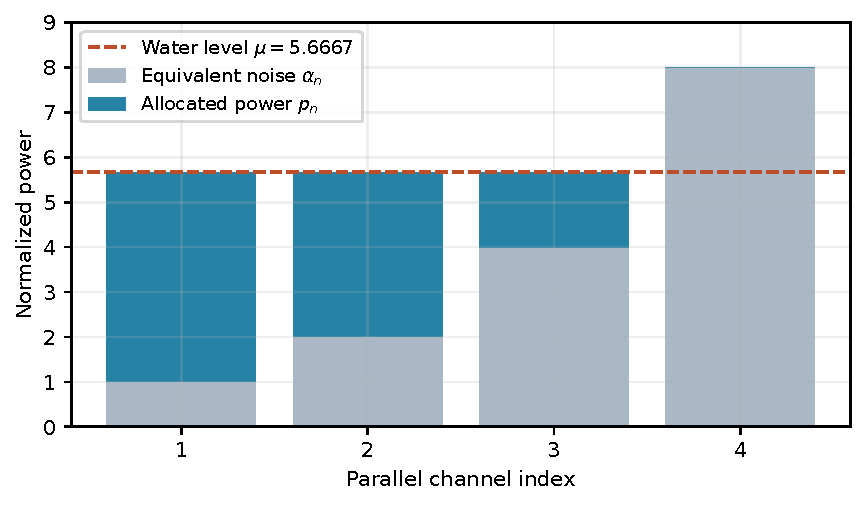
\includegraphics[width=.75\linewidth]{water_filling.pdf}
 \caption{四个单位带宽正交信道的注水分配。灰色为归一化等效噪声功率 $\alpha_n$，蓝色为分配功率 $p_n$，虚线为水位 $\mu=17/3$。总分配功率为 $10$；第四个信道的噪声底超过水位，分配功率为零。}
 \label{fig:water-numeric}
\end{figure}

\section{功率控制：谱半径条件与实际预算共同决定可行性}

三个同频链路的功率增益、噪声功率及预算取
\begin{equation}
 G=\begin{bmatrix}1&.15&.1\\.2&1&.15\\.1&.2&1\end{bmatrix},\qquad
 \sigma_k^2=.1,\quad 0\le p_k\le1,\quad\sum_kp_k\le2.
 \label{eq:numeric-power-data}
\end{equation}
要求所有链路的 SINR 至少为 $2$ 时，最小功率为
\begin{equation}
 \bm p^\star=(.462686567,.537313433,.507462687)^\T.
\end{equation}
此时 $\rho(F)=.602486<1$，三个 SINR 约束均取等号。闭式解
$(I-F)^{-1}\bm\eta$ 与 LP 解的最大分量差为 $2.44\times10^{-12}$；把 LP 解代回原 SINR 不等式、峰值与总功率约束，最大正违约量为 $1.35\times10^{-12}$。

逐步提高共同目标 $\gamma$ 时，总功率预算先限制性能。用闭式最小功率作为可行性判据，从可行下界 $0$ 和不可行上界 $10$ 开始二分，30 次后得到
\begin{equation}
 2.2170723043\le\gamma^\star\le2.2170723137.
\end{equation}
下界对应功率约为 $(.609406,.716203,.674392)^\T$，总和约为 $2$，单用户峰值仍有余量。代码还在此区间两侧各距 $10^{-3}$ 的目标处调用 LP 交叉检查可行与不可行状态；使用该间隔是为避开有限精度求解器对边界附近状态的敏感性。最终窄区间来自闭式判据，并未把求解器状态误当成无限精度证明。

\begin{figure}[H]
 \centering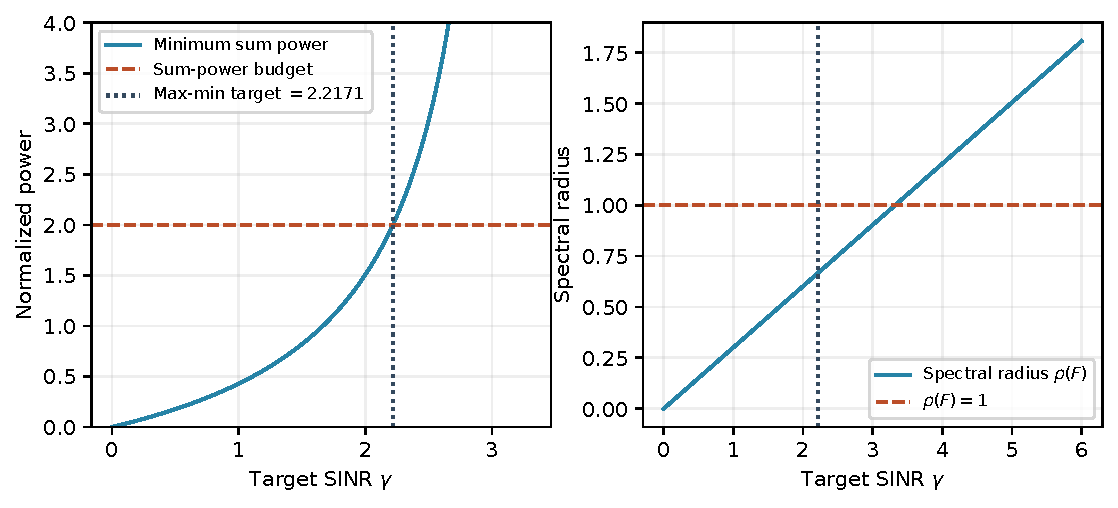
\includegraphics[width=.9\linewidth]{power_control.pdf}
 \caption{式~\eqref{eq:numeric-power-data} 的共同 SINR 目标扫描，步长为 $.02$。左图为仅考虑 SINR 时的最小总功率（纵轴显示到 $4$），水平虚线是总功率预算 $2$；右图为相应 $F$ 的谱半径。竖线标出实际预算下的最大共同 SINR。$\rho(F)<1$ 保证无预算时存在有限功率解；加入功率预算后，可行范围进一步缩小。}
 \label{fig:power-numeric}
\end{figure}

\section{WMMSE：单调上升仍可能到达不同解}

实幅度三用户干扰信道取
\begin{equation}
 H=\begin{bmatrix}1&.8&.3\\.7&1&.6\\.4&.5&1\end{bmatrix},\quad
 \sigma_k^2=.2,\quad \sum_k v_k^2\le3.
\end{equation}
仍采用复基带单位带宽速率模型；实数是本算例对信道系数和幅度的取值限制。这里 $v_k\ge0$ 是发射幅度，功率为 $p_k=v_k^2$；SINR 中的增益为 $|H_{kj}|^2$。三个用户权重均为 $1$，目标为同频链路的和频谱效率
$\sum_k\log_2(1+\SINR_k)$。固定接收器和 MSE 权重后，幅度更新的功率乘子用 80 次二分求得。迭代在相邻目标增量不超过
$10^{-10}\max(1,|R|)$ 时停止，最多 3000 次。

等功率初值和随机种子 $7$ 生成的正初值分别在 59、64 次迭代后到达约
数值 $4.597239615$（单位 bit/s/Hz），对应功率约为
$(1.3618,0,1.6382)^\T$。偏向第二个用户的初始功率
$(.01,2.98,.01)^\T$ 则在 15 次迭代后到达约
$4.000000000\,\mathrm{bit/s/Hz}$。三条轨迹均单调上升，但后者停在性能较低的解；因此“迭代不再改善”不能替代全局最优性证书。

为提供独立参照，代码枚举功率单纯形
$p_1+p_2+p_3=3$ 上步长为 $.02$ 的 11476 个点，最好可行点为
$(1.36,0,1.64)^\T$，目标为 $4.597239011$。只检查总功率取满的点有依据：正噪声下，把任意非零功率向量共同放大至预算边界，会严格改善各活跃链路的 SINR。有限网格给出的是可行目标，即全局最大值的下界；它没有覆盖所有连续功率分配，因而不是最优值上界。

\begin{figure}[H]
 \centering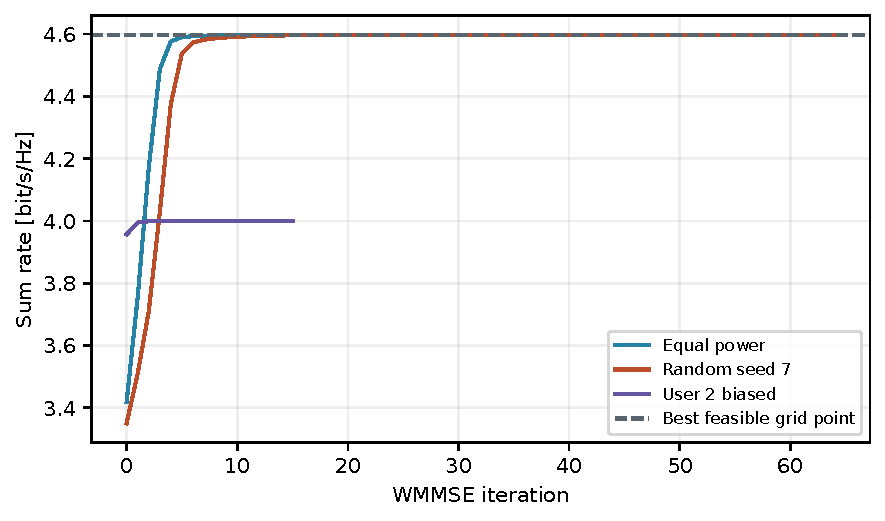
\includegraphics[width=.8\linewidth]{wmmse.pdf}
 \caption{三用户实 SISO 信道的 WMMSE 和频谱效率轨迹。随机初值由种子 $7$ 生成；偏置初值的功率为 $(.01,2.98,.01)^\T$。虚线为步长 $.02$ 的功率网格中最好可行点的目标，仅作数值参照。各条曲线在达到停止条件后结束。}
 \label{fig:wmmse-numeric}
\end{figure}

\section{稀疏估计：目标解得准与信道估得准是两件事}

实信道观测取 $\bm y=A\bm h+\bm n$：$A\in\R^{40\times80}$ 的元素由标准高斯分布生成后逐列归一化，$\bm h$ 只有 5 个非零分量，噪声标准差为 $.02$。所有随机量由同一 NumPy 生成器、种子 $7$ 顺序产生；非零位置及观测矩阵另存于数据文件。求解
\begin{equation}
 \min_{\bm x}\ \frac12\norm{A\bm x-\bm y}_2^2+.06\norm{\bm x}_1.
\end{equation}
ISTA 步长为 $1/L$，其中 $L=\norm{A}_2^2=5.310545$。以近端梯度映射的无穷范数小于 $10^{-8}$ 为停止条件，210 步后目标约为 $.2690157144$，与 CVXPY 参考目标的绝对差约 $1.52\times10^{-11}$；近端梯度映射范数为 $9.31\times10^{-9}$。这一数值证据说明优化问题已被高精度求解。

相对信道估计误差 $\norm{\widehat{\bm h}-\bm h}_2/\norm{\bm h}_2$ 仍约为 $6.71\%$。噪声和 $\ell_1$ 正则化带来的收缩偏差不会随着优化迭代继续增加而消失。选择正则化参数需要考虑噪声与估计任务，单看优化目标下降曲线不足以确定它。

\begin{figure}[H]
 \centering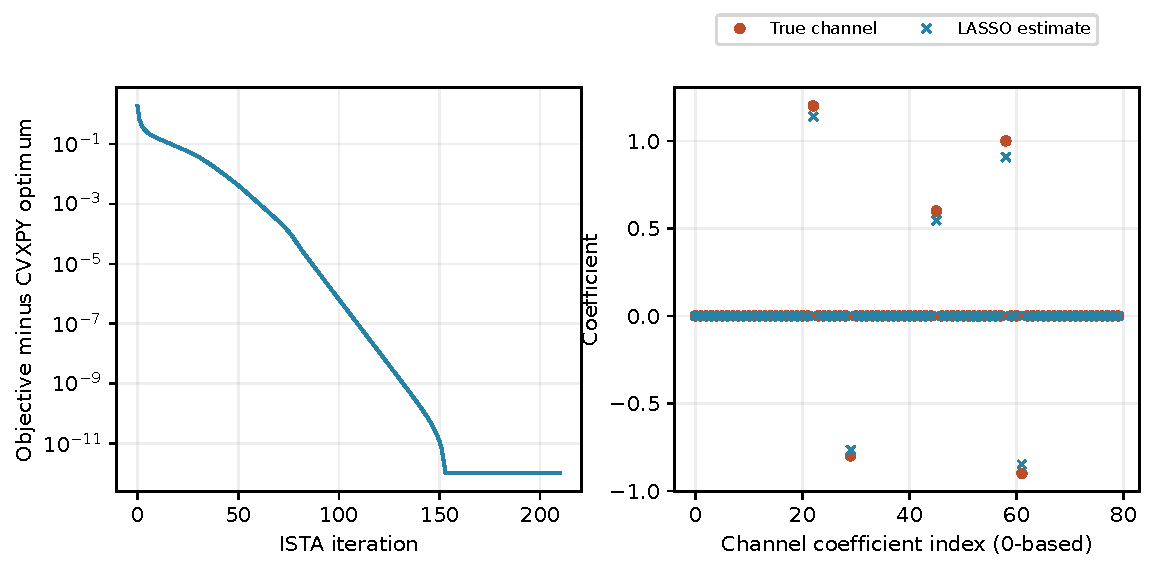
\includegraphics[width=.9\linewidth]{lasso.pdf}
 \caption{种子 $7$ 的稀疏信道估计。左图为 ISTA 目标减去 CVXPY 参考目标，作图时把小于 $10^{-12}$ 的差截至 $10^{-12}$，以容纳数值误差和对数坐标；右图为真实系数与 LASSO 估计，横轴沿用代码的零起始索引。列归一化矩阵尺寸为 $40\times80$，非零系数数目为 5，$\lambda=.06$，噪声标准差为 $.02$。}
 \label{fig:lasso-numeric}
\end{figure}

\section{复现与结果文件}

在已安装依赖的 Python 环境中，从教材根目录执行
\begin{lstlisting}
python code/run_experiments.py
\end{lstlisting}
即可重新生成全部四组图形与数据；编译教材时直接使用已附的 PDF 图，无需运行 Python。代码中包含闭式解对照、功率可行性和 WMMSE/ISTA 单调性断言。若断言不通过，应检查版本与数值状态后再解释图形。

本次运行使用 Python 3.12.14、NumPy 2.3.5、SciPy 1.17.0、CVXPY 1.9.3、Matplotlib 3.10.8 和 CLARABEL 0.11.1。凸子问题的绝对、相对间隙和可行性容差均设为 $10^{-10}$。完整参数与诊断保存在
\texttt{data/results.json}；迭代历史及系数保存在 CSV，稀疏观测输入保存在
\texttt{data/lasso\_input.npz}。版本变化可能影响最后几位数值，判断结论时应同时比较目标、原约束残差和停止准则。

\chapter{习题：从识别结构到检查解答}
\label{ch:exercises}
\chaptertakeaway{用十四道自拟习题检查建模、等价变换和算法保证。先独立完成，再对照附录中的推导；计算结果应同时满足原问题的约束。}

题目中的功率除特别说明外均已归一化。自然对数记作 $\ln$，以 $2$ 为底的对数记作 $\log_2$。建议先做题~\ref{ex:units}--\ref{ex:soc}，再做其余题目。

\begin{enumerate}[label=\textbf{\arabic*.},ref=\arabic*,itemsep=10pt]
\item \label{ex:units}\textbf{速率中的单位与带宽。}
一条复基带 AWGN 链路的接收功率增益为 $g=10^{-8}$，发射功率为 $p=0.1\,\mathrm W$，带宽为 $B=10^6\,\mathrm{Hz}$。本题把噪声功率谱密度定义为 $N_0=10^{-17}\,\mathrm{W/Hz}$，故带内噪声为 $N_0B$。
写出信噪比和速率（$\mathrm{bit/s}$），并计算数值。若把 $B$ 加倍而保持 $p,g,N_0$ 不变，信噪比和速率各怎样变化？把 $\log_2$ 换成 $\ln$ 后，如何恢复原速率？

\item \label{ex:nonconcave}\textbf{干扰破坏联合凹性。}
两个用户的噪声功率均为 $1$，直接增益均为 $1$，交叉增益均为 $2$，且 $p_1,p_2\geq0$、$p_1+p_2\leq1$。总速率为
\[
 R(p_1,p_2)=\ln\!\left(1+\frac{p_1}{1+2p_2}\right)
 +\ln\!\left(1+\frac{p_2}{1+2p_1}\right).
\]
比较 $(1,0)$、$(0,1)$ 与其中点，证明 $R$ 不是联合凹函数。为什么“每个用户的速率对自身功率是凹的”不足以证明总问题是凸优化？

\item \label{ex:water}\textbf{用 KKT 条件算一次注水。}
求解 $\max_{p\geq0}\sum_{i=1}^4\ln(1+p_i/\alpha_i)$，约束为 $\sum_i p_i\leq10$，其中 $\alpha=(1,2,4,8)$。推导水位表达式，确定激活信道，给出最优功率与总功率约束的乘子，并检查未激活信道的 KKT 不等式。

\item \label{ex:power}\textbf{固定 SINR 的线性规划与谱半径。}
两用户的增益矩阵为 $G=\left[\begin{smallmatrix}1&0.2\\0.2&1\end{smallmatrix}\right]$，噪声为 $(0.1,0.1)$，目标 SINR 都是 $2$。写出最小总功率的线性规划，构造 $p\geq Fp+u$，计算 $\rho(F)$ 与分量最小可行功率。如果每个用户的峰值功率为 $0.3$，问题是否可行？

\item \label{ex:soc}\textbf{波束成形为什么能转成二阶锥？}
单播下行的第 $k$ 个用户满足
\[
 \frac{|h_k^{\HH}w_k|^2}{\sum_{j\ne k}|h_k^{\HH}w_j|^2+\sigma_k^2}\geq\gamma_k>0.
\]
在目标为总发射功率、其他约束只与各波束的二次幅度有关时，证明可以令 $h_k^{\HH}w_k$ 为非负实数，并写出等价的二阶锥约束。若同一波束同时服务多个用户，为什么这一论证通常不能直接套用？

\item \label{ex:robust}\textbf{范数球的不确定性。}
实向量 $a=\hat a+\delta$ 满足 $\|\delta\|_2\leq\varepsilon$。证明要求 $a^{\T}x\leq b$ 对所有允许的 $\delta$ 成立，等价于
$\hat a^{\T}x+\varepsilon\|x\|_2\leq b$。给出最坏误差方向，并说明 $x=0$ 的情形。

\item \label{ex:prox}\textbf{实数与复数软阈值。}
对 $v\in\C$ 和 $\lambda\geq0$，求
$\argmin_{z\in\C}\{\frac12|z-v|^2+\lambda|z|\}$。
解释为什么最优解与非零的 $v$ 同相，并给出 $v=3+4\mathrm i$、$\lambda=2$ 的答案。它怎样退化为实数软阈值？

\item \label{ex:dual}\textbf{对偶更新的符号。}
考虑 $\min_{x\in\mathcal X} f(x)$，约束 $g(x)\leq0$，拉格朗日函数为 $L(x,\lambda)=f(x)+\lambda g(x)$。令 $x^t$ 精确最小化 $L(x,\lambda^t)$。写出对偶变量的投影更新，并解释在约束违反时乘子怎样变化。若约束改为 $a^{\T}x\geq b$，如何保持符号一致？

\item \label{ex:sca}\textbf{切线的方向决定近似是否可行。}
设 $g,h$ 均为可微凸函数。对最小化 $g(x)-h(x)$，说明应线性化哪一项，以及所得近似是原目标的上界还是下界。对约束 $g(x)-h(x)\leq0$，用同样构造得到的是内近似还是外近似？说明目标单调改进、停点和全局最优这三者的区别。

\item \label{ex:wmmse}\textbf{标量 WMMSE 恒等式。}
设 $y=as+\eta$，其中 $s,\eta$ 均为零均值，$\E|s|^2=1$，$\E[\eta s^*]=0$，$\E|\eta|^2=I>0$。用 $\hat s=u^*y$ 估计 $s$，定义 $e(u)=\E|\hat s-s|^2$。求 $u$、$e$ 的最优值，并证明
\[
 \max_{u\in\C,\,v>0}\{\ln v-ve(u)+1\}=\ln(1+|a|^2/I).
\]
这里的最优 $v$ 是什么？此恒等式本身是否证明多用户加权和速率能求得全局最优？

\item \label{ex:ee}\textbf{单链路能效与 Dinkelbach。}
对 $p_c>0$ 和 $0\leq p\leq P$，最大化归一化能效
$\eta(p)=\ln(1+p)/(p_c+p)$。推导内部最优点的方程，证明无功率上界时根唯一，并求 $p_c=1,P=4$ 的最优解。写出 Dinkelbach 子问题及 $q>0$ 时的闭式解。

\item \label{ex:assignment}\textbf{什么时候可以直接松弛指派变量？}
两个用户、两个资源块的收益矩阵为
$C=\left[\begin{smallmatrix}4&3\\3&0\end{smallmatrix}\right]$。每个用户和资源块恰好匹配一次，求最大收益匹配。解释为什么标准指派问题把 $x_{kn}\in\{0,1\}$ 松弛为 $x_{kn}\geq0$ 仍存在整数最优解。再给出增加一个线性耦合约束后出现严格松弛间隙的例子。

\item \label{ex:chance}\textbf{单个高斯约束与联合机会约束。}
令实随机向量 $a\sim\mathcal N(\mu,\Sigma)$，且 $x$ 为确定的设计变量。对 $0<\epsilon<1/2$，把
$\Prob(a^{\T}x\leq b)\geq1-\epsilon$ 写成确定性二阶锥约束。若有 $m$ 个事件、要求同时满足的概率至少为 $1-\epsilon$，怎样分配各事件的失败概率才能得到充分条件？每个事件分别满足概率 $0.95$，是否足以保证联合概率 $0.95$？

\item \label{ex:admm}\textbf{ADMM 应检查什么？}
对共识问题 $\min f(x)+g(z)$、约束 $x=z$，写出原始残差和对偶残差。当 $x^t=z^t$ 但 $z^t$ 仍明显变化时，能否停止？说明标准凸 ADMM 收敛论证通常需要什么条件；将一个模块换成非凸神经网络后，哪些保证需要重新证明？
\end{enumerate}

\appendix
\chapter{习题参考解答}
\label{app:solutions}
这些解答给出判断依据和关键计算。凡是通过变换求解的题目，最后都回到原约束检查结果。

\section*{题~\ref{ex:units}：单位与带宽}
接收信号功率为 $gp=10^{-9}\,\mathrm W$，带内噪声为 $N_0B=10^{-11}\,\mathrm W$，故信噪比为 $100$，即 $20\,\mathrm{dB}$。速率是
\[
 R=B\log_2\!\left(1+\frac{gp}{N_0B}\right)
 =10^6\log_2(101)\approx6.6582\times10^6\,\mathrm{bit/s}.
\]
带宽加倍后信噪比降为 $50$，速率为 $2\times10^6\log_2(51)\approx11.3449\times10^6\,\mathrm{bit/s}$。带宽增加既增加每秒自由度，也增加噪声；在固定总功率下速率并不按带宽成倍增加。自然对数计算的速率为 $\mathrm{nat/s}$，除以 $\ln2$ 才得到 $\mathrm{bit/s}$。

\section*{题~\ref{ex:nonconcave}：联合凹性的反例}
两个端点的总速率均为 $\ln2\approx0.6931$；中点的值为 $2\ln(5/4)\approx0.4463$，小于端点值的平均数，违反凹函数的不等式。固定他人功率后对自身功率的凹性，只描述一个坐标方向。联合凹性要求任意两个可行功率向量之间都满足凹性不等式，交叉干扰会破坏这一要求。因此最大化此总速率不构成凹目标最大化的凸优化问题。

\section*{题~\ref{ex:water}：注水与互补松弛}
最大化目标严格凹且各分量单调增加，故最优时用完功率。把问题写成负目标的最小化，乘子 $\lambda\geq0$ 对应总功率，$\nu_i\geq0$ 对应 $-p_i\leq0$，驻点条件为
\[
 -\frac1{\alpha_i+p_i}+\lambda-\nu_i=0,
 \qquad \nu_i p_i=0.
\]
正功率信道满足 $p_i=1/\lambda-\alpha_i$，故 $p_i=[\mu-\alpha_i]_+$，其中水位 $\mu=1/\lambda$。若前三条信道激活，$3\mu-(1+2+4)=10$，得到
\[
 \mu=\frac{17}{3},\qquad
 p^*=\left(\frac{14}{3},\frac{11}{3},\frac{5}{3},0\right),
 \qquad\lambda=\frac3{17}.
\]
水位位于 $4$ 和 $8$ 之间，激活集合自洽。第四条信道的乘子为 $\nu_4=3/17-1/8=7/136>0$，满足 KKT 条件。严格凹性保证上述可行 KKT 解唯一。

\section*{题~\ref{ex:power}：最小可行功率}
SINR 约束等价于 $p_1\geq0.4p_2+0.2$、$p_2\geq0.4p_1+0.2$。最小化 $p_1+p_2$，再加上非负及峰值约束，就是线性规划。这里
\[
 F=\begin{bmatrix}0&0.4\\0.4&0\end{bmatrix},\qquad
 u=\begin{bmatrix}0.2\\0.2\end{bmatrix},\qquad
 \rho(F)=0.4<1.
\]
无峰值约束时，分量最小可行功率为 $(I-F)^{-1}u=(1/3,1/3)^{\T}$。直接代入得 $(1/3)/(0.2/3+0.1)=2$。任何可行向量都不小于这个分量最小解，因此峰值为 $0.3$ 时不可行。

\section*{题~\ref{ex:soc}：相位选择与锥约束}
把 $w_k$ 乘以单位模复数 $\exp[-\mathrm i\arg(h_k^{\HH}w_k)]$，可使其期望信号为非负实数。该操作保持所有 $|h_\ell^{\HH}w_k|$、$\|w_k\|_2$ 不变；题设的目标和约束因此均不改变。固定相位后原约束等价于
\[
 \left\|\begin{bmatrix}(h_k^{\HH}w_j)_{j\ne k}\\\sigma_k\end{bmatrix}\right\|_2
 \leq\frac{\Rea(h_k^{\HH}w_k)}{\sqrt{\gamma_k}},
 \qquad \Ima(h_k^{\HH}w_k)=0.
\]
右侧由锥约束自动要求非负。复向量的范数可用其实部、虚部的堆叠表示成实二阶锥。多播时同一个 $w$ 同时出现在多个期望信号 $h_k^{\HH}w$ 中；一个整体相位通常无法让它们全部为非负实数，因此不能由此得到相同的等价凸化。

\section*{题~\ref{ex:robust}：最坏误差的方向}
由 Cauchy--Schwarz 不等式，$\delta^{\T}x\leq\varepsilon\|x\|_2$。当 $x\ne0$ 时，取 $\delta=\varepsilon x/\|x\|_2$ 即达到上界，故
\[
 \max_{\|\delta\|_2\leq\varepsilon}(\hat a+\delta)^{\T}x
 =\hat a^{\T}x+\varepsilon\|x\|_2.
\]
最坏误差沿着使左端增长最快的方向。这证明了鲁棒约束的等价形式。若 $x=0$，最大值为 $0$，任意允许误差均达到该值，约束退化为 $0\leq b$。

\section*{题~\ref{ex:prox}：复数软阈值}
若 $v\ne0$，固定 $|z|=r$ 后，$|z-v|^2=r^2+|v|^2-2\Rea(z^*v)$ 在 $z$ 与 $v$ 同相时最小。剩下的标量问题是
$\min_{r\geq0}\frac12(r-|v|)^2+\lambda r$，其解为 $r=[|v|-\lambda]_+$。于是
\[
 \prox_{\lambda|\cdot|}(v)=
 \begin{cases}
 (1-\lambda/|v|)v,&|v|>\lambda,\\
 0,&|v|\leq\lambda.
 \end{cases}
\]
给定数值的答案为 $\frac35(3+4\mathrm i)=1.8+2.4\mathrm i$。当 $v\in\R$ 时，它成为 $\operatorname{sign}(v)[|v|-\lambda]_+$；$v=0$ 时解为 $0$。

\section*{题~\ref{ex:dual}：对偶上升而非下降}
对偶函数 $d(\lambda)=\inf_{x\in\mathcal X}L(x,\lambda)$ 为凹函数，所需步骤是最大化它。若 $x^t$ 是精确最小解，$g(x^t)$ 是其超梯度，故
\[
 \lambda^{t+1}=[\lambda^t+\eta_t g(x^t)]_+,
 \qquad\eta_t>0.
\]
约束违反时 $g(x^t)>0$，乘子增加，使后续原变量更新对违反约束付出更大代价。约束 $a^{\T}x\geq b$ 应先写成 $b-a^{\T}x\leq0$，相应更新使用 $b-a^{\T}x^t$。只有写清拉格朗日函数，才可确定更新符号。

\section*{题~\ref{ex:sca}：上界与内近似}
凸函数满足
$h(x)\geq h(x^t)+\nabla h(x^t)^{\T}(x-x^t)$，因此
\[
 g(x)-h(x)\leq
 g(x)-h(x^t)-\nabla h(x^t)^{\T}(x-x^t)
 =:\widetilde f(x;x^t).
\]
应线性化被减去的 $h$。最小化这个凸上界，若它在 $x^t$ 处取等，且新点使上界不增，就有 $f(x^{t+1})\leq f(x^t)$。把 $\widetilde f(x;x^t)\leq0$ 用作约束给出内近似：满足新约束必满足原约束，并保留当前可行点。

单调有界只保证目标值收敛，尚不能保证迭代点收敛。要得到聚点为停点，还需梯度一致、适当的紧致性或有界性、约束正则性以及对子问题的求解精度等条件。停点是一阶条件；非凸目标的不同停点可能有不同目标值，不能由单调性或停点条件推出全局最优。

\section*{题~\ref{ex:wmmse}：先优化接收器，再优化权重}
由不相关性，误差为
\[
 e(u)=|u|^2(|a|^2+I)-2\Rea(u^*a)+1.
\]
配方得到 $u_{\mathrm{opt}}=a/(|a|^2+I)$，$e_{\min}=I/(|a|^2+I)=1/(1+|a|^2/I)>0$。对固定 $e>0$，函数 $\ln v-ve+1$ 关于 $v>0$ 严格凹，其导数为 $1/v-e$，故最大值在 $v=1/e$，值为 $-\ln e$。再最小化误差即得题中恒等式，联合最优权重为 $v_{\mathrm{opt}}=1+|a|^2/I$。

该恒等式给出一种精确的目标重写。多用户中对波束、接收器和权重轮流优化，一般只解联合非凸问题的各个子问题；恒等式并未赋予这些交替迭代全局最优保证。

\section*{题~\ref{ex:ee}：唯一根与能效参数}
分母始终为正，故导数的符号由
\[
 H(p)=\frac{p_c+p}{1+p}-\ln(1+p)
\]
决定。它满足 $H(0)=p_c>0$、$H'(p)=-(p_c+p)/(1+p)^2<0$，且 $H(p)\to-\infty$。因此存在唯一正根 $p_0$，目标先增后减；有上界时最优功率为 $\min(P,p_0)$。内部最优条件为
\[
 (1+p_0)\ln(1+p_0)=p_c+p_0.
\]
当 $p_c=1$ 时 $p_0=\mathrm e-1\approx1.71828<4$，最优能效为 $1/\mathrm e$，单位为归一化的 $\mathrm{nat/J}$。

Dinkelbach 子问题为 $\max_{0\leq p\leq P}\{\ln(1+p)-q(p_c+p)\}$。当 $q>0$，最优解是 $p(q)=\min\{P,\max\{0,1/q-1\}\}$；当 $q=0$ 时取 $P$。每轮更新 $q\leftarrow\ln(1+p(q))/(p_c+p(q))$。以子问题最优值接近零作为停止依据；它为零时恰好满足分式问题的全局最优条件。

\section*{题~\ref{ex:assignment}：指派多面体与耦合约束}
两个整数匹配分别是对角线匹配，收益 $4$，以及交叉匹配，收益 $6$，故后者最优。标准指派问题的约束矩阵是全幺模的，右端为整数；其可行多面体的极点为整数，线性目标因此存在整数最优解。最优解存在不意味着每个最优解都必须是整数。

增加耦合约束 $x_{12}+x_{21}\leq1$。所有满足行列和为 $1$ 的二阶矩阵均可写为
\[
 X=\begin{bmatrix}t&1-t\\1-t&t\end{bmatrix},\qquad 0\leq t\leq1.
\]
新约束为 $t\geq1/2$，目标为 $6-2t$。松弛最优解取 $t=1/2$，收益 $5$；整数可行解只能取 $t=1$，收益 $4$，出现严格间隙。新增约束可能破坏原来的整数极点结构。

\section*{题~\ref{ex:chance}：高斯分位数与失败概率预算}
标量 $a^{\T}x$ 均值为 $\mu^{\T}x$，方差为 $x^{\T}\Sigma x$。取 $\Sigma=LL^{\T}$，并令 $\Phi$ 为标准正态分布函数。所求等价约束为
\[
 \mu^{\T}x+\Phi^{-1}(1-\epsilon)\|L^{\T}x\|_2\leq b.
\]
因 $\epsilon<1/2$，分位数为正，约束为凸二阶锥形式。零方差时随机量退化成常数，原约束直接等价于 $\mu^{\T}x\leq b$，上式仍成立。

对第 $j$ 个事件分配 $0<\epsilon_j<1/2$，令 $\sum_j\epsilon_j\leq\epsilon$，再逐个保证失败概率不超过 $\epsilon_j$。并集界给出联合失败概率不超过总预算，无需事件独立。若两个成功事件独立且概率均为 $0.95$，联合概率仅为 $0.95^2=0.9025$，所以单独的 $0.95$ 保证不足以推出联合的 $0.95$。

\section*{题~\ref{ex:admm}：两个残差都要小}
共识形式常用的残差是 $r^t=x^t-z^t$ 和 $s^t=\rho(z^t-z^{t-1})$，其中 $\rho>0$ 是固定罚参数。原始残差衡量共识约束，对偶残差反映对偶最优性条件中的不一致。当 $r^t=0$ 但 $s^t$ 仍大时，尚不能按标准残差准则停止；阈值应同时含绝对项和相对项，以适应变量维数和尺度。

标准两块凸 ADMM 的典型论证要求 $f,g$ 为闭、真、凸函数，问题存在鞍点，采用相应形式的精确子问题更新并固定正罚参数；原始、对偶残差收敛并不自动保证所有原变量序列唯一收敛。引入非凸神经网络后，凸性和精确求解等条件可能不成立，须针对新模型重证有界性、下降或其他控制关系、聚点的可行性与停点性质。不能直接沿用凸 ADMM 的全局最优保证。

\chapter{速查：表示、求解与阅读路线}\label{ch:reference}

\section{复数模型如何交给实数求解器}
通信模型常用复数简化记号，优化的凸性仍是在实数坐标下判断。若 $z=x+\mathrm i y$，其等价实向量是 $\widetilde z=[x^{\T},y^{\T}]^{\T}$；复矩阵 $A$ 的实表示为
\begin{equation}
 \widetilde A=\begin{bmatrix}\Rea A&-\Ima A\\\Ima A&\Rea A\end{bmatrix},\qquad
 \norm{Az-b}_2=\norm{\widetilde A\widetilde z-\widetilde b}_2.
\end{equation}
若 $Q=Q^{\HH}$，则 $z^{\HH}Qz=\widetilde z^{\T}\widetilde Q\widetilde z$。这不是把复变量简单“取实部”；虚部仍是完整决策变量。

对实值函数 $f(z)$，实微分为 $\mathrm df=\nabla_x f^{\T}\mathrm dx+\nabla_y f^{\T}\mathrm dy$。若采用 Wirtinger 记号，则
\begin{equation}
 \frac{\partial f}{\partial z^*}=\frac12(\nabla_x f+\mathrm i\nabla_y f).
\end{equation}
例如 $f(z)=\norm{Az-b}_2^2$ 的 $\partial f/\partial z^*=A^{\HH}(Az-b)$，而实坐标梯度对应 $2A^{\HH}(Az-b)$。实现中的步长要与梯度约定一致。第4、5章使用 $\tfrac12\norm{Az-b}_2^2$ 的近端梯度时，实坐标更新对应 $A^{\HH}(Az-b)$。

\section{稳健二次约束与 S 引理}
范数不确定性不仅出现在线性支持函数中，也出现在二次服务质量约束。一个重要工具是 S 引理。令实向量 $e\in\R^n$ 满足 $\norm e_2\le\epsilon$，$\epsilon>0$。对实对称 $Q$、向量 $b$ 与标量 $c$，下式的稳健约束
\begin{equation}\label{eq:slemma-quad}
 e^{\T}Qe+2b^{\T}e+c\ge0\quad\text{对所有 }\norm e_2\le\epsilon
\end{equation}
等价于存在 $\lambda\ge0$ 使
\begin{equation}\label{eq:slemma-lmi}
 \begin{bmatrix}Q+\lambda I&b\\b^{\T}&c-\lambda\epsilon^2\end{bmatrix}\succeq0.
\end{equation}
这将无限多条约束变成有限维 SDP 约束。充分性可直接核验：式\eqref{eq:slemma-lmi} 表示对任意 $e$，二次式\eqref{eq:slemma-quad}的左侧加 $\lambda(\norm e_2^2-\epsilon^2)$ 非负；在球内第二项非正，所以原二次式非负。必要性来自单个严格可行二次约束下的 S 引理；这里 $e=0$ 严格位于球内，满足其条件\cite{ben2009}。多个二次不确定约束同时出现时，同样加多个乘子的做法通常仅是充分条件。

在通信中可以先把最坏信道下的 SINR 门限写成关于信道误差的二次式，再应用此式。若 $Q,b,c$ 对协方差设计变量仿射，所得矩阵不等式保持凸性；若它们还含有变量乘积，则引入 S 引理并不会自动消除剩余非凸性。矩阵是 Hermitian 的复数版本也可用相应复 S 引理，或先转为实数表示并核对不确定集合。

\section{一页算法选择表}
\begingroup\small
\begin{longtable}{p{.24\textwidth}p{.30\textwidth}p{.35\textwidth}}
\toprule 识别出的结构 & 优先选择 & 应报告的保证或证据\\\midrule\endhead
少数可消元的资源变量 & KKT、单调根搜索、注水 & 方程残差、边界分支与全局条件\\
固定 SINR 功控 & LP、谱半径检验 & 原可行残差、最小功率、不可行原因\\
单流单播功率最小化 & 相位固定后的 SOCP & 等价性、原 SINR 核验\\
凸光滑大规模模型 & 投影梯度、加速梯度 & 步长依据、梯度映射或函数界\\
凸光滑加可近端正则 & ISTA/FISTA、ADMM & 目标与残差、凸问题的精度指标\\
中等规模凸锥模型 & 内点法/锥求解器 & 原对偶间隙和锥约束残差\\
干扰和速率 & SCA、WMMSE & 可行性、真实目标、多初值和驻点误差\\
单个能效比值 & Dinkelbach & 子问题全局条件和参数残差\\
单位模、秩一限制 & 流形/相位法、SDR & 可实施性，恢复目标与松弛界\\
固定收益匹配 & 指派算法、LP 极点 & 整数最优解和等价性\\
一般离散耦合 & 分支定界、有效松弛 & 可行目标、全局界、gap、时限\\
随机信道长期设计 & SAA、随机梯度 & 抽样分布、验证样本、统计误差\\
在线队列决策 & 漂移加惩罚、受约束 MDP & 稳定性条件、成本/积压权衡\\\bottomrule
\end{longtable}
\endgroup

\section{继续学习时怎样选资料}
希望补强凸分析与对偶，可读 Boyd--Vandenberghe\cite{boyd2004}；希望把算法与无线链路模型连起来，可读 Tse--Viswanath\cite{tse2005}。理解 SDP 松弛的条件与随机恢复，读 Luo 等的教程\cite{luo2010}；理解非凸块更新的驻点结论，读 Razaviyayn 等\cite{razaviyayn2013}；理解长期性能与队列权衡，读 Neely\cite{neely2010}。

遇到新场景，先用第1章的地图检查新增变量、耦合和信息时序，再核验所选方法的条件。

\backmatter
\begin{thebibliography}{99}
\addcontentsline{toc}{chapter}{参考文献}
\small

\bibitem{boyd2004}
S. Boyd and L. Vandenberghe.
\emph{Convex Optimization}. Cambridge University Press, 2004.
\href{https://web.stanford.edu/~boyd/cvxbook/}{作者提供的书籍与配套资源}。

\bibitem{cvxexamples}
CVX Research and example contributors.
\emph{CVX Example Library}, 包含 A. Mutapcic 编写的功率控制与阵列设计示例，2006。
本书核查版本：\href{https://github.com/cvxr/CVX/tree/a0a775908bc1eec1625d56498d0224132b0d8b7f/examples}{CVX commit a0a7759}。
\href{https://github.com/cvxr/CVX/blob/a0a775908bc1eec1625d56498d0224132b0d8b7f/LICENSE.txt}{许可证中 Example library 小节}将示例库列为公有领域；核查日期 2026-11-08。

\bibitem{cvxpyexamples}
R. Gowers, R. Hill, S. Al-Izzi, T. Pollington, and K. Briggs.
\emph{Water Filling in Communications};
\emph{Power Assignment in a Wireless Communication System}.
CVXPY 官方示例，\href{https://github.com/cvxpy/examples/tree/73a6892ef5bea4ded68f8f9fab17e48119dc62f5/notebooks/WWW}{核查版本 commit 73a6892，2026}。
\href{https://github.com/cvxpy/examples/blob/73a6892ef5bea4ded68f8f9fab17e48119dc62f5/LICENSE}{Apache-2.0}；核查日期 2026-11-08。

\bibitem{tse2005}
D. Tse and P. Viswanath.
\emph{Fundamentals of Wireless Communication}.
Cambridge University Press, 2005.
\href{https://web.stanford.edu/~dntse/wireless_book.html}{作者提供的在线章节}。

\bibitem{yates1995}
R. D. Yates.
A framework for uplink power control in cellular radio systems.
\emph{IEEE Journal on Selected Areas in Communications}, 13(7):1341--1347, 1995.
\href{https://doi.org/10.1109/49.414651}{doi:10.1109/49.414651}.

\bibitem{kelly1998}
F. P. Kelly, A. K. Maulloo, and D. K. H. Tan.
Rate control for communication networks: shadow prices, proportional fairness and stability.
\emph{Journal of the Operational Research Society}, 49(3):237--252, 1998.
\href{https://www.statslab.cam.ac.uk/~fpk1/rate.html}{作者论文主页}。

\bibitem{lebret1997}
H. Lebret and S. Boyd.
Antenna array pattern synthesis via convex optimization.
\emph{IEEE Transactions on Signal Processing}, 45(3):526--532, 1997.
\href{https://web.stanford.edu/~boyd/papers/ant-pat.html}{作者论文主页}。

\bibitem{luo2010}
Z.-Q. Luo, W.-K. Ma, A. M.-C. So, Y. Ye, and S. Zhang.
Semidefinite relaxation of quadratic optimization problems.
\emph{IEEE Signal Processing Magazine}, 27(3):20--34, 2010.
\href{https://doi.org/10.1109/MSP.2010.936019}{doi:10.1109/MSP.2010.936019}.

\bibitem{ben2009}
A. Ben-Tal, L. El Ghaoui, and A. Nemirovski.
\emph{Robust Optimization}.
Princeton University Press, 2009.
\href{https://press.princeton.edu/books/ebook/9781400831050/robust-optimization-pdf}{出版社书籍页面}。

\bibitem{shi2011}
Q. Shi, M. Razaviyayn, Z.-Q. Luo, and C. He.
An iteratively weighted MMSE approach to distributed sum-utility maximization for a MIMO interfering broadcast channel.
\emph{IEEE Transactions on Signal Processing}, 59(9):4331--4340, 2011.
\href{https://doi.org/10.1109/TSP.2011.2147784}{doi:10.1109/TSP.2011.2147784}.

\bibitem{shen2018}
K. Shen and W. Yu.
Fractional programming for communication systems---Part I: Power control and beamforming.
\emph{IEEE Transactions on Signal Processing}, 66(10):2616--2630, 2018.
\href{https://doi.org/10.1109/TSP.2018.2812733}{doi:10.1109/TSP.2018.2812733}.

\bibitem{dinkelbach1967}
W. Dinkelbach.
On nonlinear fractional programming.
\emph{Management Science}, 13(7):492--498, 1967.
\href{https://doi.org/10.1287/mnsc.13.7.492}{doi:10.1287/mnsc.13.7.492}.

\bibitem{razaviyayn2013}
M. Razaviyayn, M. Hong, and Z.-Q. Luo.
A unified convergence analysis of block successive minimization methods for nonsmooth optimization.
\emph{SIAM Journal on Optimization}, 23(2):1126--1153, 2013.
\href{https://doi.org/10.1137/120891009}{doi:10.1137/120891009}.

\bibitem{beck2009}
A. Beck and M. Teboulle.
A fast iterative shrinkage-thresholding algorithm for linear inverse problems.
\emph{SIAM Journal on Imaging Sciences}, 2(1):183--202, 2009.
\href{https://doi.org/10.1137/080716542}{doi:10.1137/080716542}.

\bibitem{boyd2011}
S. Boyd, N. Parikh, E. Chu, B. Peleato, and J. Eckstein.
Distributed optimization and statistical learning via the alternating direction method of multipliers.
\emph{Foundations and Trends in Machine Learning}, 3(1):1--122, 2011.
\href{https://web.stanford.edu/~boyd/papers/admm_distr_stats.html}{作者论文与配套实现主页}。

\bibitem{neely2010}
M. J. Neely.
\emph{Stochastic Network Optimization with Application to Communication and Queueing Systems}.
Morgan \& Claypool, 2010.
\href{https://doi.org/10.2200/S00271ED1V01Y201006CNT007}{doi:10.2200/S00271ED1V01Y201006CNT007}.

\bibitem{writing2026}
hongjinrui.
\emph{科研写作（research-writing）规则}, 2026.
\href{https://github.com/hongjinrui/writing_skills/blob/main/SKILL.md}{SKILL.md}。
本书采用其符号定义、推导衔接、假设与证据、图表可复现等写作规则；读取日期 2026-11-08。

\bibitem{shapiro2009}
A. Shapiro, D. Dentcheva, and A. Ruszczy\'nski.
\emph{Lectures on Stochastic Programming: Modeling and Theory}.
SIAM and MPS, 2009.
\href{https://doi.org/10.1137/1.9780898718751}{doi:10.1137/1.9780898718751}.

\bibitem{puterman1994}
M. L. Puterman.
\emph{Markov Decision Processes: Discrete Stochastic Dynamic Programming}.
Wiley, 1994.
\href{https://doi.org/10.1002/9780470316887}{doi:10.1002/9780470316887}.
\end{thebibliography}

\end{document}
